\documentclass{article}

% Essential packages
\usepackage{graphicx}   % For image handling
\usepackage{subcaption} % For multi images
\usepackage{caption}    % For proper captions
\usepackage{listings}   % For code listings
\usepackage{fontspec}   % For custom fonts
\usepackage{xcolor}     % For color support
\usepackage{tcolorbox}  % For code block boxes
\usepackage{etoolbox}   % For patching and command manipulation
\usepackage{titlesec}   % For section formatting
\usepackage{parskip}    % For customisable paragraph formating
\usepackage{comment}    % For being able to comment out sections
\usepackage{geometry}   % For managing page size and margins
\usepackage{hyperref}   % For embedding links, like URL's
\usepackage{bigstrut}
\usepackage{multirow}
\usepackage{colortbl}
\usepackage{amsmath}    % For math and equation formatting

\tcbuselibrary{listings, skins, breakable}  %Librarary to make code blocks multipage


%   ############################## Customisation ##############################

% Document metadata
\title{\fontsize{24}{36}\selectfont PB1140V - Elektrisitetslære 2\\ %Edit title here \\ means new line
Lab 06} % Line 2 of title, its not subtitle, that is possible to, google it
\author{Sølve Kjelseth} % Input your name
\date{\today} % Auto updates the date, untill you export it, replace with hardcoded date if you need

% Adjust the body text font size to 12pt without affecting section headings
\renewcommand{\normalsize}{\fontsize{12}{16}\selectfont}

% Adjust the paragraph spacing, either as indentation or/and line spaceing
\setlength{\parindent}{0pt}  % Remove indentation
\setlength{\parskip}{6pt}    % Add vertical space between paragraphs

% Customisation of fonts and colors
\setmainfont{Times New Roman}
\setmonofont{JetBrains Mono}
\definecolor{background}{RGB}{225, 219, 202}
\definecolor{darkAccent}{RGB}{140, 98, 64}
\definecolor{commentGreen}{RGB}{26, 159, 32}
\definecolor{keywordPurple}{RGB}{229, 24, 192}
\definecolor{keywordBlue}{RGB}{5, 142, 217}
\definecolor{portOrange}{RGB}{234, 72, 31}
\definecolor{darkGray}{RGB}{60, 60, 60}

% Link color customization
\hypersetup{
    colorlinks=true,
    linkcolor=darkGray, % Internal links such as table of contents or figure referencing
    urlcolor=keywordBlue % URL colors
    }
\urlstyle{same} % Makes url in the same style as the rest of the document

% Customisation of margins and paper size
\geometry{
 a4paper,
 left = 30mm,
 right = 30mm,
 top = 30mm,
 bottom = 30mm
 }

% Sections formatting and numbering
% Sets the font to monospace for section, subsection and subsubsection
% and sets the format to be numbers with . between and at the end
\renewcommand{\thesection}{\texttt{\arabic{section}.}}
\renewcommand{\thesubsection}{\texttt{\arabic{section}.\arabic{subsection}.}}
\renewcommand{\thesubsubsection}{\texttt{\arabic{section}.\arabic{subsection}.\arabic{subsubsection}.}}

\setcounter{section}{-1}  % Start section numbering from 0, delete this to start from 1

% Makes section monospace font and start each subsection from 0 and figure number
\let\oldsection\section
\renewcommand{\section}[1]{%
  \oldsection{\texttt{#1}} % Make section title monospace
  \setcounter{subsection}{-1} % Makes subsection start from 0, delete this line to start from 1
  \setcounter{figure}{-1} % Makes figure numbers start from 0, delete this line to start from 1
  \setcounter{table}{-1} % Makes table numbers start from 0, delete this line to start from 1
}


% Makes subsection monospace font and start each subsubsection from 0
\let\oldsubsection\subsection
\renewcommand{\subsection}[1]{%
  \oldsubsection{\texttt{#1}}% Make subsection title monospace
  \setcounter{subsubsection}{-1}% Makes subsubsection start from 0, delete this line to start from 1
}

% Makes subsubsection monospace font
\let\oldsubsubsection\subsubsection
\renewcommand{\subsubsection}[1]{%
  \oldsubsubsection{\texttt{#1}}% Make subsubsection title monospace
}

% Makes every new section start on a new page, except for the first section, section 0
\pretocmd{\section}{%
  \ifnum\value{section}=-1 \else\clearpage\fi % Replace -1 with 0 if sections start at nr. 1
}{}{}

% Makes Table of contents a subsection
\makeatletter
\renewcommand{\tableofcontents}{%
    \subsection{Table of Contents} % Numbered subsection named Table of contents
    \@starttoc{toc}%
}
\makeatother

% Makes List of figures a subsection
\makeatletter
\renewcommand{\listoffigures}{%
    \subsection{List of Figures} % Numbered subsection named List of figures
    \@starttoc{lof}%
}
\makeatother

% Makes List of tables a subsection
\makeatletter
\renewcommand{\listoftables}{%
    \subsection{List of Tables} % Numbered subsection named List of tables
    \@starttoc{lot}%
}
\makeatother

% Makes every figure be formated as section number.figure number
\renewcommand{\thefigure}{\arabic{section}.\arabic{figure}}

% Makes every table be formated as section number.table number
\renewcommand{\thetable}{\arabic{section}.\arabic{table}}
\AtBeginEnvironment{tabular}{\ttfamily} % Monozpaced font within tables

% Add keywords to be highlited in blue below. Note that all reserved
% keywords from VHDL is already in purple and should not be added here
% too as duplicates will cause issues. Therfore compile this document
% after pasting in code and only add non-highlited words to this list.
% Also, there is not a list for orange keywords, used for ports here.
\lstdefinelanguage{VHDL+}{
    language     = VHDL,
    morestring = [b]',
    morekeywords = [2]{
        IEEE,
        std_logic_1164, std_logic, std_logic_vector},
    morekeywords = [3]{
        SW, LEDR, KEY,
        HEX0, HEX1, HEX2, HEX3, HEX4, HEX5, HEX6},
    sensitive = false
}


%   ############################## Advanced customisation ##############################

% Customisation of list style inside code block
\lstdefinestyle{VHDL}{
    language = VHDL+, % Uses the extra higlights from above
    % The folloowing lines defines color for highlighting, other changes like
    % italic, bold or different fonts can also be added to this
    commentstyle = \color{commentGreen}, 
    keywordstyle = \color{keywordPurple},
    keywordstyle = [2]\color{keywordBlue},
    keywordstyle = [3]\color{portOrange},
    stringstyle = \color{darkAccent},
    basicstyle = \ttfamily\small, % Default font inside code block
    numberstyle = \ttfamily\color{darkAccent}, % Style of line numbering
    numbers = left, % Line numbering on left side
    breakatwhitespace = false, % Don't start new line with only whitspaces
    breaklines = true, % If line is to long it will wrap to next line (line number does not increase)
    keepspaces = true, % Indents works logical
    showspaces = false, % Space is blank character, set to true to show dots instad
    showstringspaces = false, % Same as above but inside strings
    showtabs = false, % Tab is also blank character, set to true to show dashes
    tabsize = 4, % Tabsize is set to 4, this works well with code from notepad++
    % Dont mess with the ones below unless you want to mess with the box as well
    % These took some time to line up such that it looks natural
    numbersep = 10pt, % Adjust distance between numbers and code
    xleftmargin = -8pt,% Negative margin to pull code text closer to the left border
}

% This is for code where VHDL is not an argument
\lstdefinestyle{Example Code}{
    basicstyle = \ttfamily\small, % Default font inside code block
    numberstyle = \ttfamily\color{darkAccent}, % Style of line numbering
    numbers = left, % Line numbering on left side
    breakatwhitespace = false, % Don't start new line with only whitspaces
    breaklines = true, % If line is to long it will wrap to next line (line number does not increase)
    keepspaces = true, % Indents works logical
    showspaces = false, % Space is blank character, set to true to show dots instad
    showstringspaces = false, % Same as above but inside strings
    showtabs = false, % Tab is also blank character, set to true to show dashes
    tabsize = 4, % Tabsize is set to 4, this works well with code from notepad++
    % Dont mess with the ones below unless you want to mess with the box as well
    % These took some time to line up such that it looks natural
    numbersep = 10pt, % Adjust distance between numbers and code
    xleftmargin = -8pt,% Negative margin to pull code text closer to the left border
}

\lstset{style = Example Code} %Sets the default style to Example Code

% Customisation of code block itself
\newtcolorbox[auto counter, number within=section]{codeBlock}[2][]{
    colback=background, % Background color for the code block
    colframe=darkAccent, % Border color for the code block
    listing only, %Makes it contain the listing
    arc=10pt, % Rounded corners size
    sharp corners=northeast, % Make top-right corner sharp for the main box
    enhanced jigsaw, % Essential dont mess with it
    breakable, % Allows content to be multipage
    top=-4pt, % Made to line up text dont mess with it
    bottom=-4pt, % Same as above
    before skip=0pt, after skip=10pt, % Adjust spacing before and after the box
    boxrule=1pt, % Border thickness of the main box
    overlay unbroken and first={\node[ % Create label box in the top-right corner
        anchor=north east,      %Position of box, same as sharp corner in this case
        fill=background,        %Background color same as main box
        draw=darkAccent,        %Outline color, same as main box
        line width=1pt,         %Outline thickness, same as main box
        text=keywordPurple,     %Text color
        font=\ttfamily,         %Text font and size
        inner sep=6pt,          %Spacing inside
        minimum width=16pt,     %Minimum box with, it autoresizes depending on text
        minimum height=12pt,    %Minimum box height, it autoresizes depending on text
        text centered,          %Centres the text with the spacing
        sharp corners]          %Makes corners sharp
        at ([xshift=0pt, yshift=0pt]frame.north east) % Position, aligned with corner on main box
        {#2}; % Types your argument in the top corner as a label
    }
}

\newcommand{\writecode}[3][Example Code]{%
    \par\medskip % Adds some vertical spacing before the caption
    \begin{center} % Center the caption
        Code \refstepcounter{figure}\thefigure: #3 % Fake caption
    \end{center}
    \label{Code:#2} % Unique label for referencing
    \addcontentsline{lof}{figure}{Code \thefigure: #3} % Manually add entry to List of Figures
    \vspace{1.5em} % Adds extra space after the caption, before the code block
    \begin{codeBlock}{#1}% arg 1 (default Example Code) will be written in the top right corner box
        \lstinputlisting[style=#1]{Code/#2}% arg 1 style is used and arg 2 is filename
    \end{codeBlock}%
}

\newcommand{\figcaption}[1]{%
    \caption[]{#1} % Suppress the default entry in LoF
    \addcontentsline{lof}{figure}{Figure \thefigure: #1} % Manually add the correct format
}

\newcommand{\tabcaption}[1]{%
    \caption[]{#1} % Suppress the default entry in LoT
    \addcontentsline{lot}{table}{Table \thetable: #1} % Manually add the correct format
}

\newcommand{\unit}[1]{\ensuremath{\, \mathrm{#1}}}



%   ############################## Document begins here ##############################

\begin{document}

\maketitle % Makes title front page based on the title, author and date metadata, change at the top


%           ########## Section ##########


\addtocontents{toc}{\protect\setcounter{tocdepth}{0}} % Temporarily hide from TOC
\section{Introduction} % Numbered section named Introduction
This is the first report in this course, detailing the completion of the lab 6  simulation exercises.
Note: All files (Excel, KiCAD, Plots) and the \LaTeX\ code for this document is open source
\href{https://github.com/Kjelseth/CircuitDesign}{github link}.
\clearpage
\tableofcontents % Generate TOC
\clearpage
\listoffigures % List of figures
\clearpage
\listoftables
\addtocontents{toc}{\protect\setcounter{tocdepth}{2}} % Restore TOC depth


%   ############################## Section ##############################
\section{Task 1}
In this task all simulations are done using the circuit in figure~\ref{fig:Circuit1}, the only thing changing is the frequency, based on the question.

\begin{figure}[h]
    \centering
    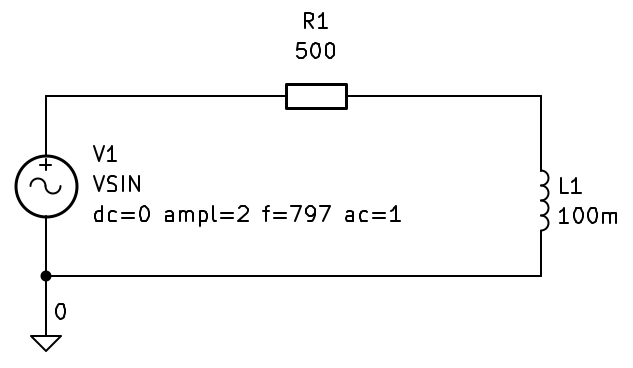
\includegraphics[width=0.8\textwidth]{Figures/Circuts/Task1.jpg}
    \figcaption{Circuit for Task 1}
    \label{fig:Circuit1}
\end{figure}

\clearpage
\subsection{a}

For all tasks the settings for the Frequency plot was the same, using values from the video instruction. \(2000\) points per decade and a frequency from \(1 \unit{Hz}\) to \(20 \unit{kHz}\).\par
Doing a frequency analysis on the circuit gives the plot in Figure~\ref{fig:Fplot1}.

\begin{figure}[h]
    \centering
    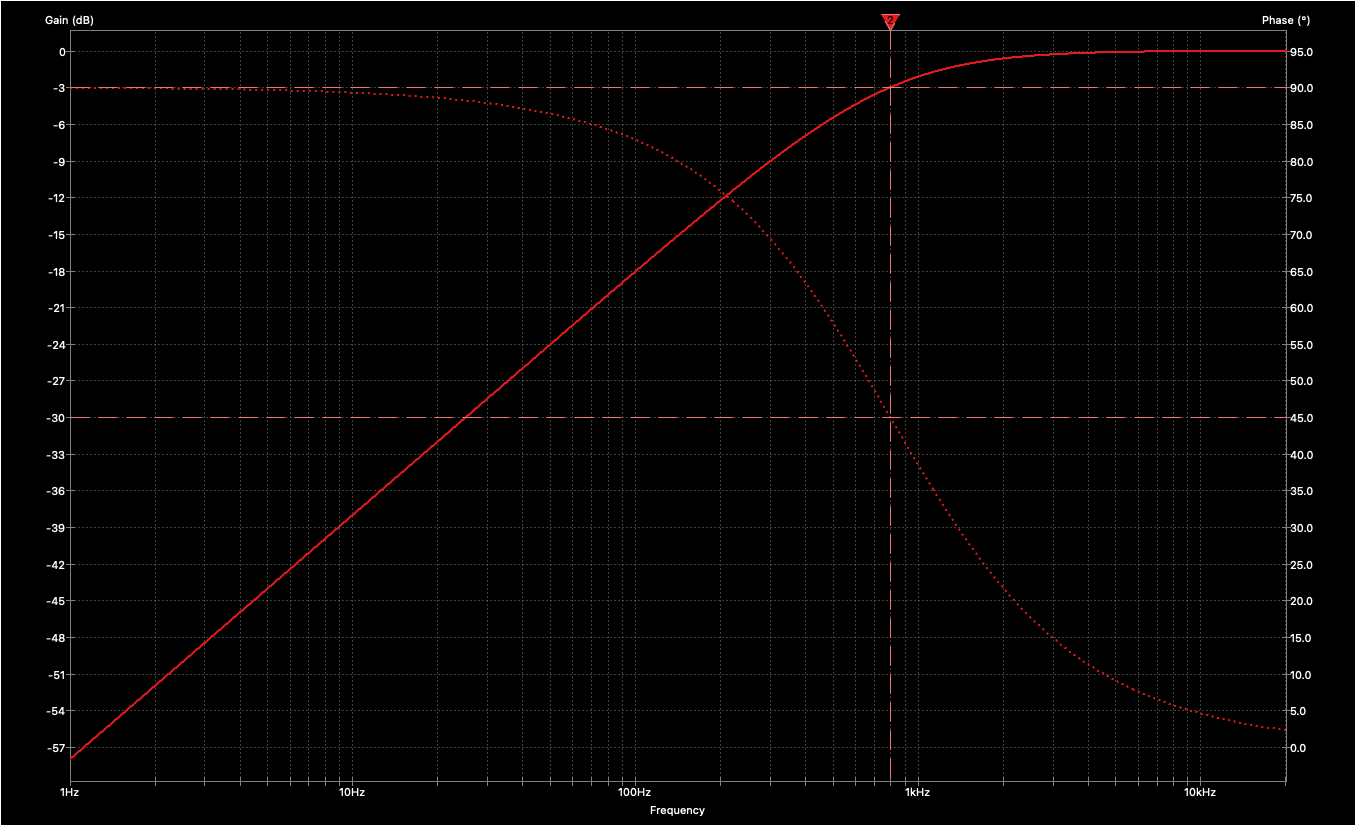
\includegraphics[width=1\textwidth]{Figures/Plots/Task1/1a-frekvens_plot.png}
    \figcaption{Frequency analysis of the circuit}
    \label{fig:Fplot1}
\end{figure}

Reading the plot at the point where the gain is at \(-3 \unit{dB}\), the resulting values for frequency and phase are found and listed in Table~\ref{tab:1a}.

% Table generated by Excel2LaTeX from sheet 'Part 1'
\begin{table}[htbp]
  \centering
  \tabcaption{Readings from plot}
    \begin{tabular}{|c|c|c|}
    \hline
    Frequency & Gain  & Phase \bigstrut\\
    \hline
    797Hz & -3dB  & 44,956° \bigstrut\\
    \hline
    \end{tabular}%
  \label{tab:1a}%
\end{table}%

\clearpage
\subsection{b}

\(F_{critical}\) is the point where the resistance is equal to the reactance, setting these equal each other, derives Equation~\ref{eq:f_L}. Using the known values of \(R\) and \(L\) the theoretical value was calculated and the simulated value was compared to it to find the deviation, listing the results in Table~\ref{tab:1b}.

\begin{equation*}
    X_L = 2 \pi f L
\end{equation*}

\begin{equation*}
    R = X_L, \text{ at } f = F_{critical}
\end{equation*}

\begin{equation*}
    R = 2 \pi F_{critical} L
\end{equation*}

\begin{equation}
    F_{critical} = \frac{R}{2 \pi L}
    \label{eq:f_L}
\end{equation}

% Table generated by Excel2LaTeX from sheet 'Part 1'
\begin{table}[htbp]
  \centering
  \tabcaption{Calculated vs Simulated frequency}
    \begin{tabular}{|c|c|c|}
    \hline
    Calculated & Simulated & Deviation \bigstrut\\
    \hline
    795,8Hz & 797Hz & 0,15\% \bigstrut\\
    \hline
    \end{tabular}%
  \label{tab:1b}%
\end{table}%

\subsection{c}

To scale the Transient plots correctly, the settings values was calculated with the equations below by following the video guide. These formulas will be used for every transient plot but for obvious reasons will only be listed once. All obtained values are found within the excel document in the \href{https://github.com/Kjelseth/CircuitDesign}{github}.

\begin{equation*}
    T = \frac{1}{f}
\end{equation*}

\begin{equation*}
    T_{step} = \frac{T}{100}
\end{equation*}

\begin{equation*}
    T_{inirial} = T
\end{equation*}

\begin{equation*}
    T_{final} = 3T
\end{equation*}

\clearpage

Performing a transient analysis using the simulated \(F_{critical}\) value, the resulting plot is shown in Figure~\ref{fig:Tplot1c}.

\begin{figure}[h]
    \centering
    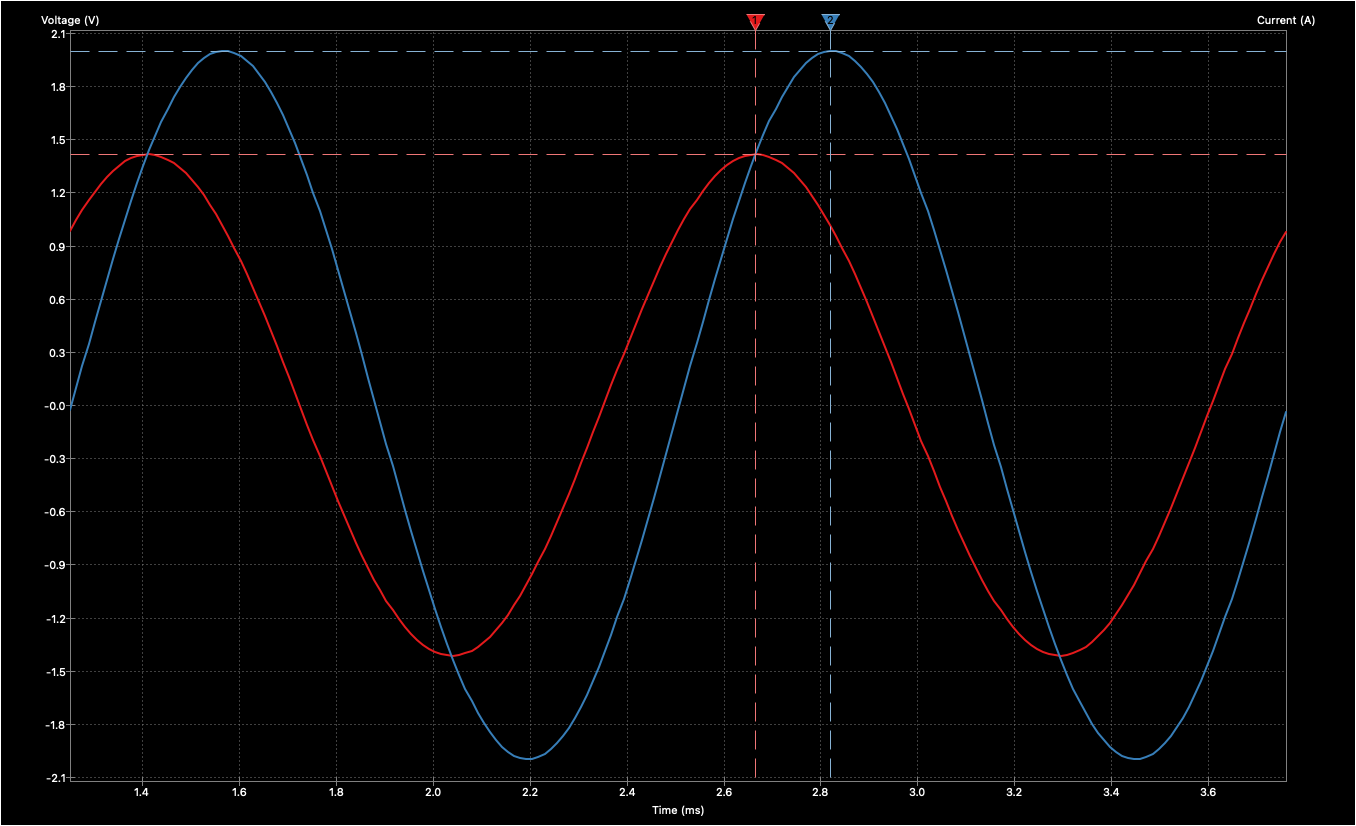
\includegraphics[width=1\textwidth]{Figures/Plots/Task1/1c-transient_plot.png}
    \figcaption{Transient analysis for 797Hz}
    \label{fig:Tplot1c}
\end{figure}

Reading the plot at the peak voltages, the resulting values and difference listed in Table~\ref{tab:1c}.

% Table generated by Excel2LaTeX from sheet 'Part 1'
\begin{table}[htbp]
  \centering
  \tabcaption{Simulated Voltages at 797Hz}
    \begin{tabular}{|c|c|c|}
    \hline
    \rowcolor[rgb]{ .753,  .902,  .961} Generator & \cellcolor[rgb]{ 1,  .592,  .584}Output & \cellcolor[rgb]{ 1,  1,  1}Difference \bigstrut\\
    \hline
    \rowcolor[rgb]{ .753,  .902,  .961} 2,00V & \cellcolor[rgb]{ 1,  .592,  .584}1,41V & \cellcolor[rgb]{ 1,  1,  1}585mV \bigstrut\\
    \hline
    \end{tabular}%
  \label{tab:1c}%
\end{table}%

\clearpage
\subsection{d}

Performing a transient analysis using a decade lower frequency than the simulated \(F_{critical}\) value, the resulting plot is shown in Figure~\ref{fig:Tplot1d}.

\begin{figure}[h]
    \centering
    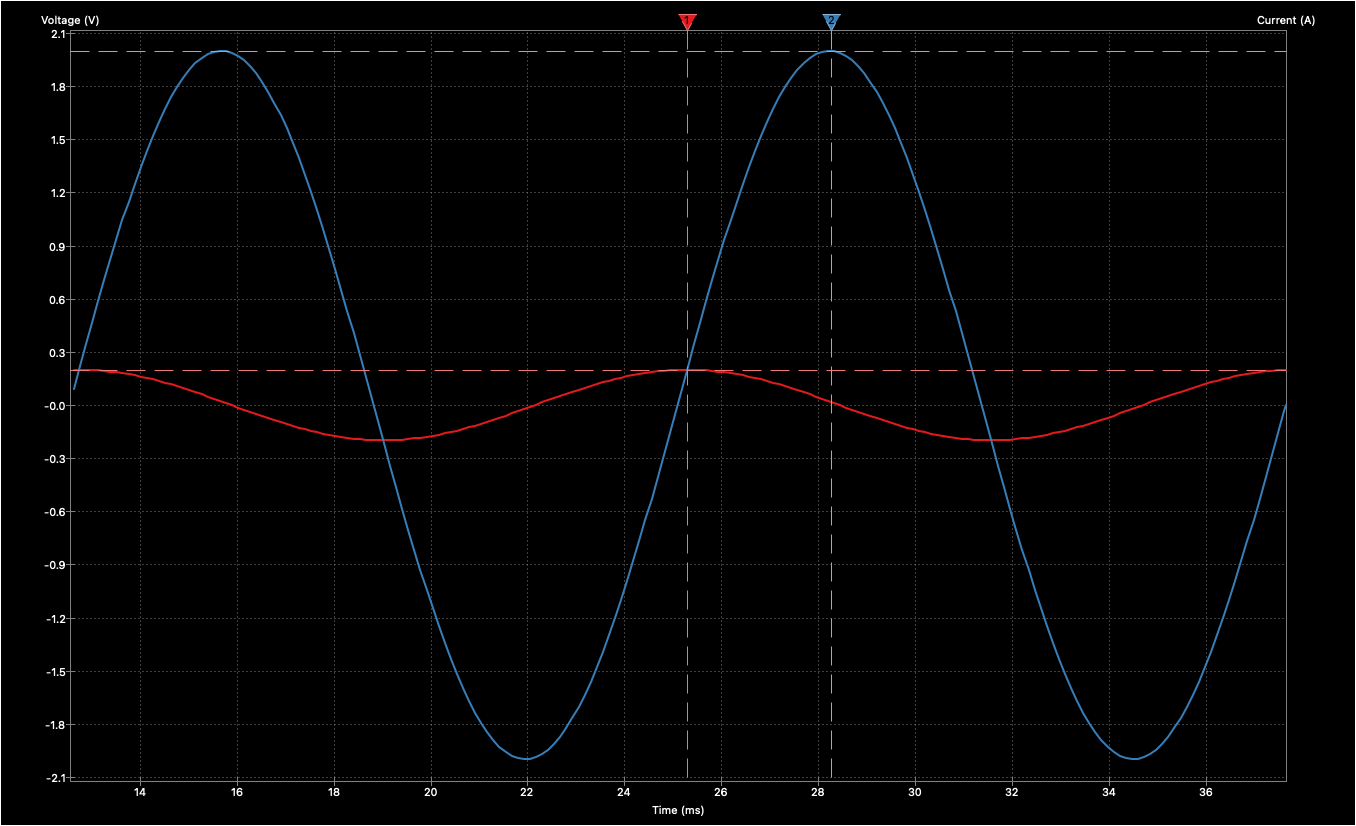
\includegraphics[width=1\textwidth]{Figures/Plots/Task1/1d-transient_plot.png}
    \figcaption{Transient analysis for 79,7Hz}
    \label{fig:Tplot1d}
\end{figure}

Reading the plot at the peak voltages, the resulting values and difference listed in Table~\ref{tab:1d}.

% Table generated by Excel2LaTeX from sheet 'Part 1'
\begin{table}[htbp]
  \centering
  \tabcaption{Simulated voltages at 79,7Hz}
    \begin{tabular}{|c|c|c|}
    \hline
    \rowcolor[rgb]{ .753,  .902,  .961} Generator & \cellcolor[rgb]{ 1,  .592,  .584}Output & \cellcolor[rgb]{ 1,  1,  1}Difference \bigstrut\\
    \hline
    \rowcolor[rgb]{ .753,  .902,  .961} 2,00V & \cellcolor[rgb]{ 1,  .592,  .584}199mV & \cellcolor[rgb]{ 1,  1,  1}1,80V \bigstrut\\
    \hline
    \end{tabular}%
  \label{tab:1d}%
\end{table}%

\clearpage
\subsection{e}

Performing a transient analysis using a decade higher frequency than the simulated \(F_{critical}\) value, the resulting plot is shown in Figure~\ref{fig:Tplot1e}.

\begin{figure}[h]
    \centering
    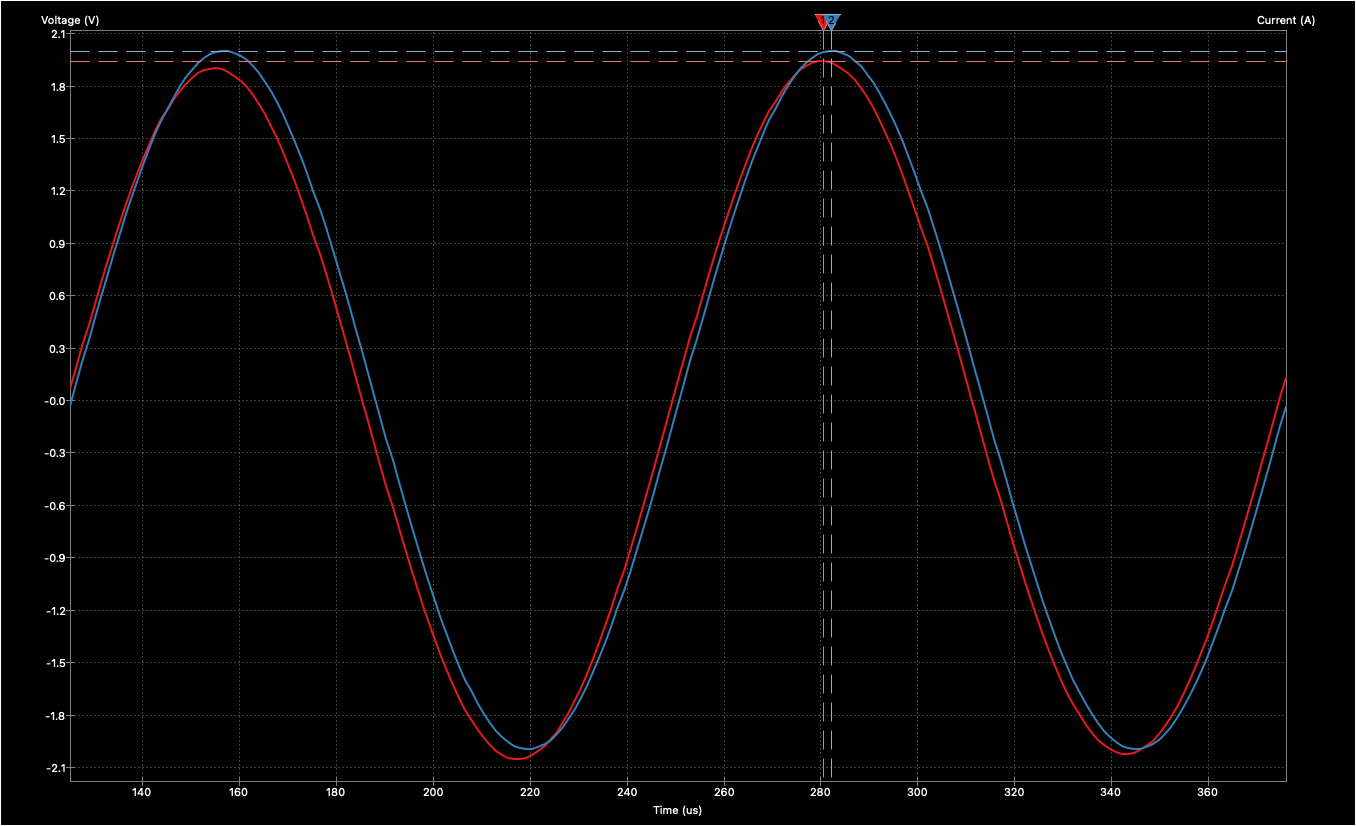
\includegraphics[width=1\textwidth]{Figures/Plots/Task1/1e-transient_plot.png}
    \figcaption{Transient analysis for 7,97kHz}
    \label{fig:Tplot1e}
\end{figure}

Reading the plot at the peak voltages, the resulting values and difference listed in Table~\ref{tab:1e}.

% Table generated by Excel2LaTeX from sheet 'Part 1'
\begin{table}[htbp]
  \centering
  \tabcaption{Simulated voltages at 7,97kHz}
    \begin{tabular}{|c|c|c|}
    \hline
    \rowcolor[rgb]{ .753,  .902,  .961} Generator & \cellcolor[rgb]{ 1,  .592,  .584}Output & \cellcolor[rgb]{ 1,  1,  1}Difference \bigstrut\\
    \hline
    \rowcolor[rgb]{ .753,  .902,  .961} 2,00V & \cellcolor[rgb]{ 1,  .592,  .584}1,94V & \cellcolor[rgb]{ 1,  1,  1}59,1mV \bigstrut\\
    \hline
    \end{tabular}%
  \label{tab:1e}%
\end{table}%


\subsection{f}
The values clearly show that the higher frequencies is almost not affected by the filer and the lower frequencies are drastically reduced, this means that this is a High-pass filter.

%   ############################## Section ##############################
\section{Task 2}

In this task all simulations are done using the circuit in figure~\ref{fig:Circuit2}, the only thing changing is the frequency, based on the question.

\begin{figure}[h]
    \centering
    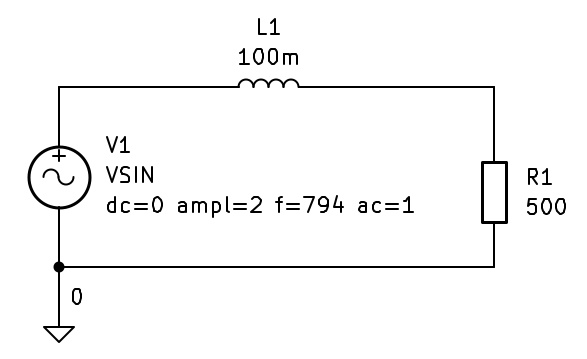
\includegraphics[width=0.8\textwidth]{Figures/Circuts/Task2.jpg}
    \figcaption{Circuit for Task 2}
    \label{fig:Circuit2}
\end{figure}

\clearpage
\subsection{a}

Doing a frequency analysis on the circuit gives the plot in Figure~\ref{fig:Fplot2}.

\begin{figure}[h]
    \centering
    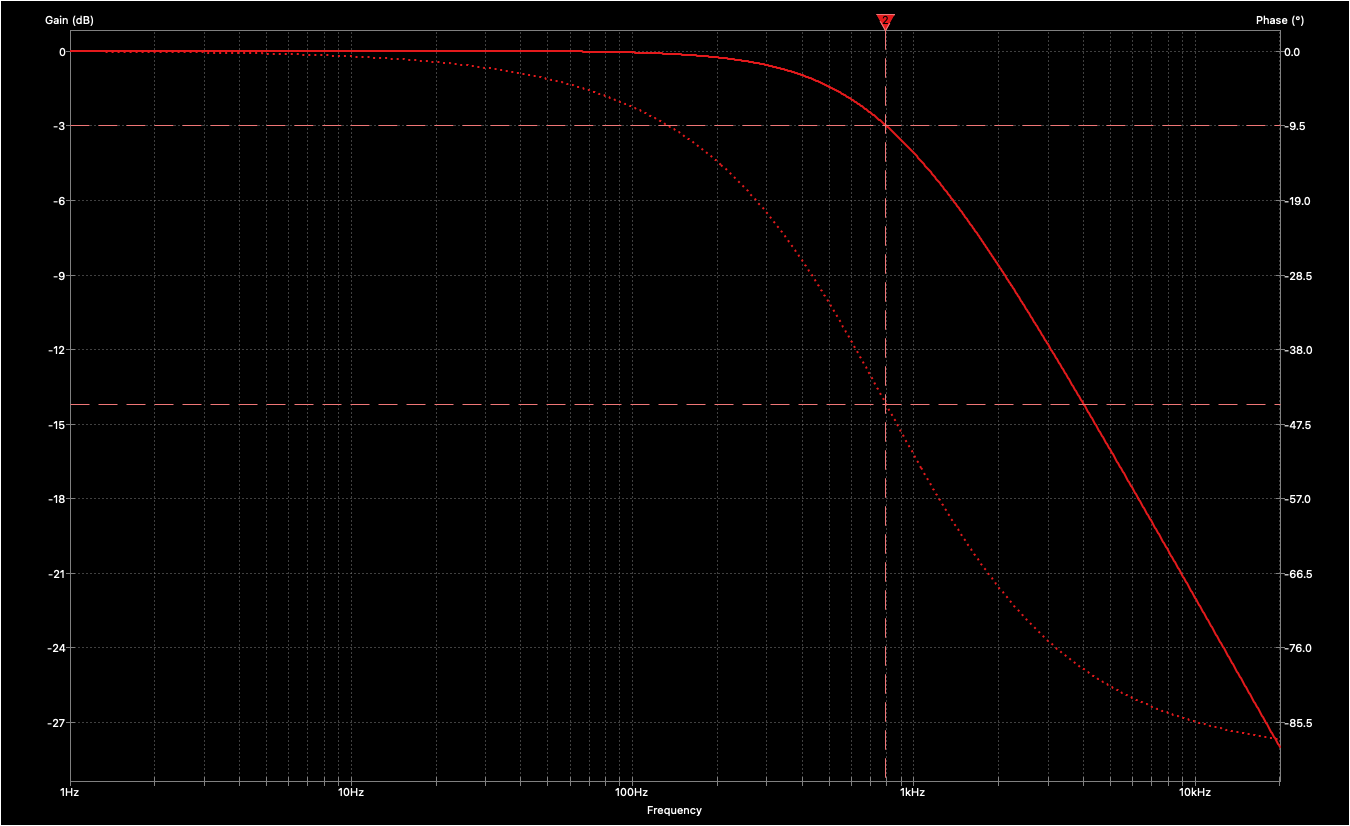
\includegraphics[width=1\textwidth]{Figures/Plots/Task2/2a-frekvens_plot.png}
    \figcaption{Frequency analysis of the circuit}
    \label{fig:Fplot2}
\end{figure}

Reading the plot at the point where the gain is at \(-3 \unit{dB}\), the resulting values for frequency and phase are found and listed in Table~\ref{tab:2a}.

% Table generated by Excel2LaTeX from sheet 'Part 2'
\begin{table}[htbp]
  \centering
  \tabcaption{Readings from plot}
    \begin{tabular}{|c|c|c|}
    \hline
    Frequency & Gain  & Phase \bigstrut\\
    \hline
    794Hz & -3dB  & -44,936° \bigstrut\\
    \hline
    \end{tabular}%
  \label{tab:2a}%
\end{table}%

\clearpage
\subsection{b}

Using the known values of \(R\) and \(L\) the theoretical value was calculated using Equation~\ref{eq:f_L}. Then the simulated value was compared to it to find the deviation, listing the results in Table~\ref{tab:2b}.

% Table generated by Excel2LaTeX from sheet 'Part 2'
\begin{table}[htbp]
  \centering
  \tabcaption{Calculated vs Simulated frequency}
    \begin{tabular}{|c|c|c|}
    \hline
    Calculated & Simulated & Deviation \bigstrut\\
    \hline
    795,8Hz & 794Hz & -0,22\% \bigstrut\\
    \hline
    \end{tabular}%
  \label{tab:2b}%
\end{table}%


\subsection{c}

Performing a transient analysis using the simulated \(F_{critical}\) value, the resulting plot is shown in Figure~\ref{fig:Tplot2c}.

\begin{figure}[h]
    \centering
    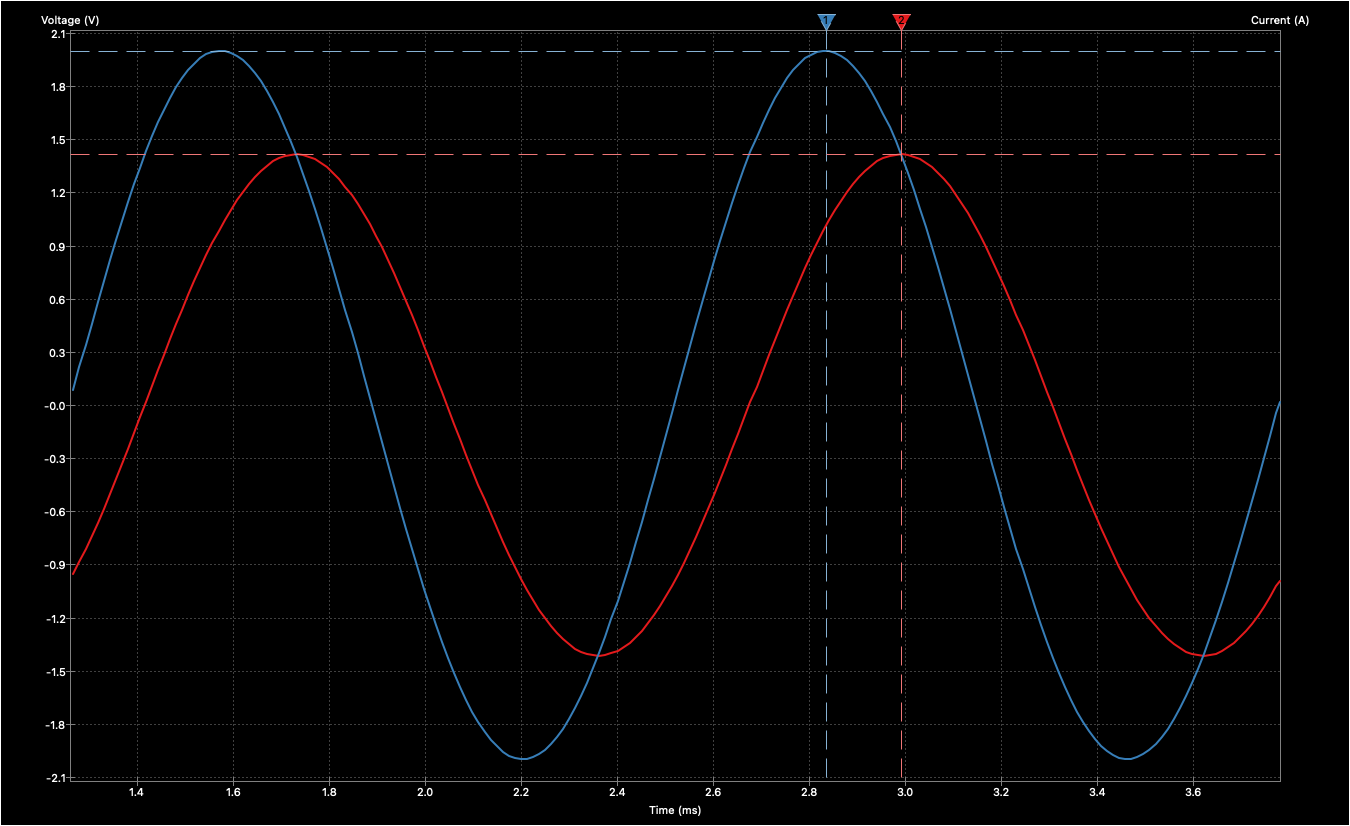
\includegraphics[width=1\textwidth]{Figures/Plots/Task2/2c-transient_plot.png}
    \figcaption{Transient analysis for 794Hz}
    \label{fig:Tplot2c}
\end{figure}

Reading the plot at the peak voltages, the resulting values and difference listed in Table~\ref{tab:2c}.

% Table generated by Excel2LaTeX from sheet 'Part 2'
\begin{table}[htbp]
  \centering
  \tabcaption{Simulated voltages at 794Hz}
    \begin{tabular}{|c|c|c|}
    \hline
    \rowcolor[rgb]{ .753,  .902,  .961} Generator & \cellcolor[rgb]{ 1,  .592,  .584}Output & \cellcolor[rgb]{ 1,  1,  1}Difference \bigstrut\\
    \hline
    \rowcolor[rgb]{ .753,  .902,  .961} 2,00V & \cellcolor[rgb]{ 1,  .592,  .584}1,42V & \cellcolor[rgb]{ 1,  1,  1}584mV \bigstrut\\
    \hline
    \end{tabular}%
  \label{tab:2c}%
\end{table}%

\clearpage
\subsection{d}

Performing a transient analysis using a decade lower frequency than the simulated \(F_{critical}\) value, the resulting plot is shown in Figure~\ref{fig:Tplot2d}.

\begin{figure}[h]
    \centering
    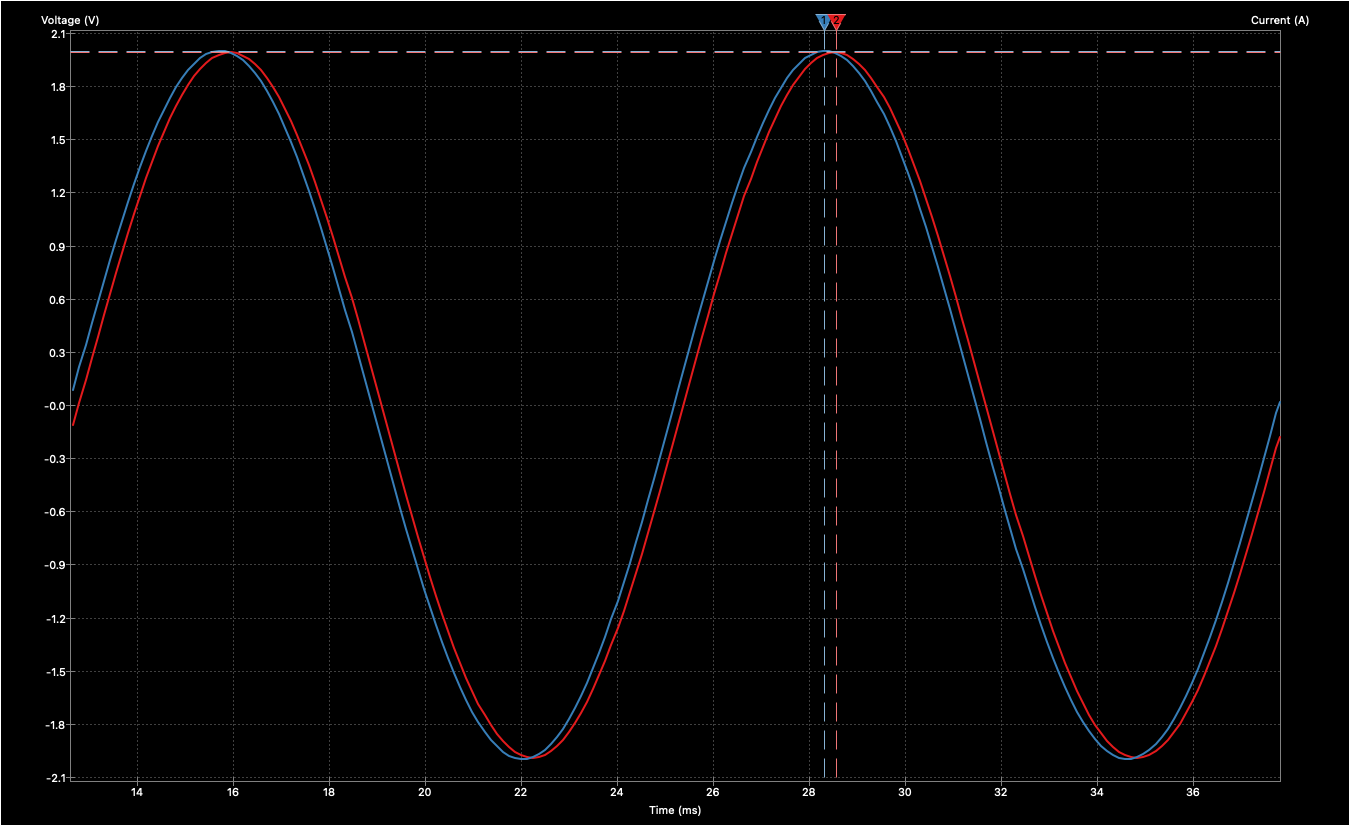
\includegraphics[width=1\textwidth]{Figures/Plots/Task2/2d-transient_plot.png}
    \figcaption{Transient analysis for 79,4Hz}
    \label{fig:Tplot2d}
\end{figure}

Reading the plot at the peak voltages, the resulting values and difference listed in Table~\ref{tab:2d}.

% Table generated by Excel2LaTeX from sheet 'Part 2'
\begin{table}[htbp]
  \centering
  \tabcaption{Simulated voltages at 79,4Hz}
    \begin{tabular}{|c|c|c|}
    \hline
    \rowcolor[rgb]{ .753,  .902,  .961} Generator & \cellcolor[rgb]{ 1,  .592,  .584}Output & \cellcolor[rgb]{ 1,  1,  1}Difference \bigstrut\\
    \hline
    \rowcolor[rgb]{ .753,  .902,  .961} 2,00V & \cellcolor[rgb]{ 1,  .592,  .584}1,99V & \cellcolor[rgb]{ 1,  1,  1}9,61mV \bigstrut\\
    \hline
    \end{tabular}%
  \label{tab:2d}%
\end{table}%

\clearpage
\subsection{e}

Performing a transient analysis using a decade higher frequency than the simulated \(F_{critical}\) value, the resulting plot is shown in Figure~\ref{fig:Tplot2e}.

\begin{figure}[h]
    \centering
    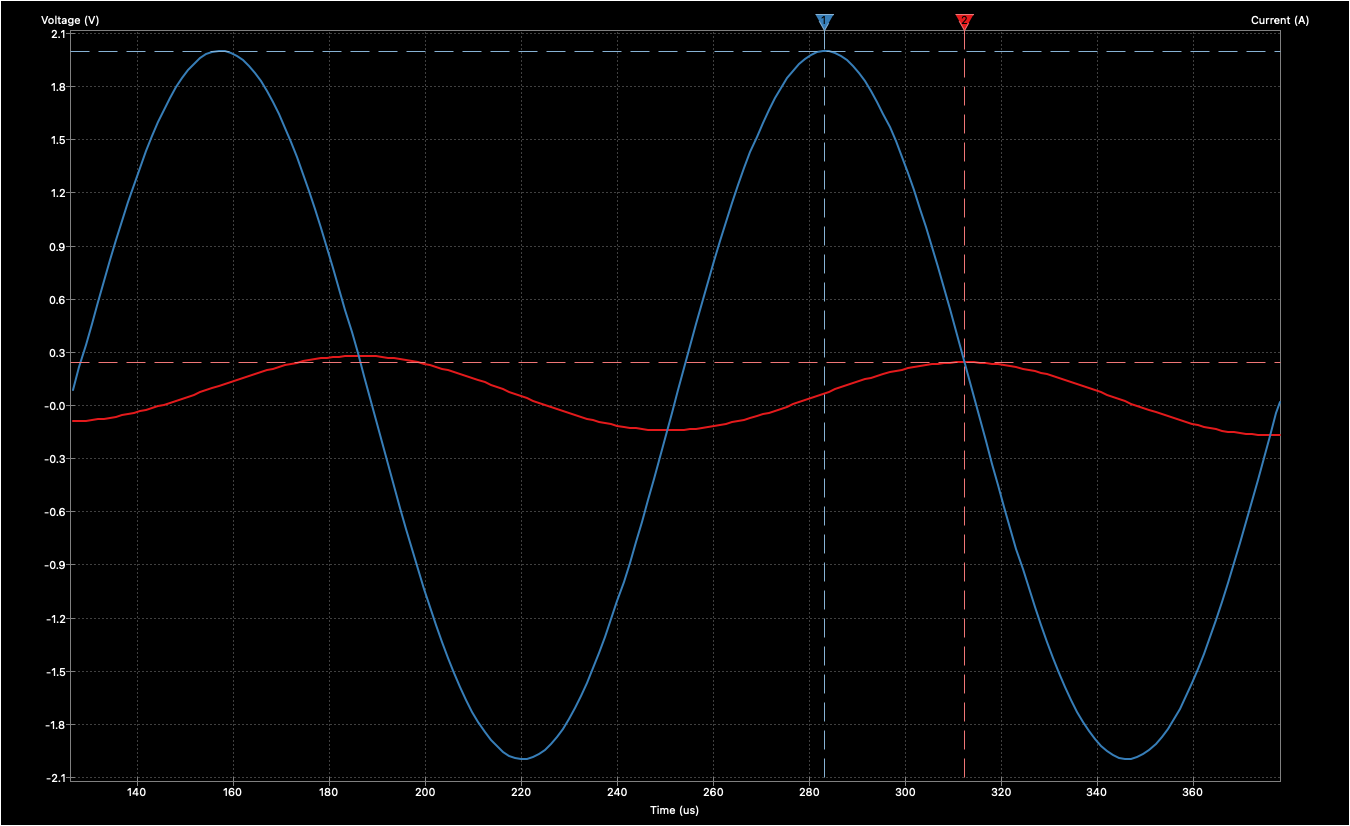
\includegraphics[width=1\textwidth]{Figures/Plots/Task2/2e-transient_plot.png}
    \figcaption{Transient analysis for 7,94kHz}
    \label{fig:Tplot2e}
\end{figure}

Reading the plot at the peak voltages, the resulting values and difference listed in Table~\ref{tab:2e}.

% Table generated by Excel2LaTeX from sheet 'Part 2'
\begin{table}[htbp]
  \centering
  \tabcaption{Simulated voltages at 7,94kHz}
    \begin{tabular}{|c|c|c|}
    \hline
    \rowcolor[rgb]{ .753,  .902,  .961} Generator & \cellcolor[rgb]{ 1,  .592,  .584}Output & \cellcolor[rgb]{ 1,  1,  1}Difference \bigstrut\\
    \hline
    \rowcolor[rgb]{ .753,  .902,  .961} 2,00V & \cellcolor[rgb]{ 1,  .592,  .584}241mV & \cellcolor[rgb]{ 1,  1,  1}1,76V \bigstrut\\
    \hline
    \end{tabular}%
  \label{tab:2e}%
\end{table}%

\subsection{f}

The values clearly show that the lower frequencies is almost not affected by the filer and the higher frequencies are drastically reduced, this means that this is a Low-pass filter.

%   ############################## Section ##############################
\section{Task 3}

In this task all simulations are done using the circuit in figure~\ref{fig:Circuit3}, the only thing changing is the frequency, based on the question.

\begin{figure}[h]
    \centering
    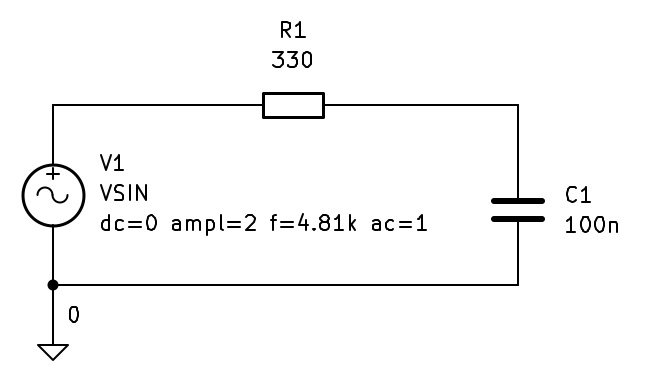
\includegraphics[width=0.8\textwidth]{Figures/Circuts/Task3.jpg}
    \figcaption{Circuit for Task 3}
    \label{fig:Circuit3}
\end{figure}

\clearpage
\subsection{a}

Doing a frequency analysis on the circuit gives the plot in Figure~\ref{fig:Fplot3}.

\begin{figure}[h]
    \centering
    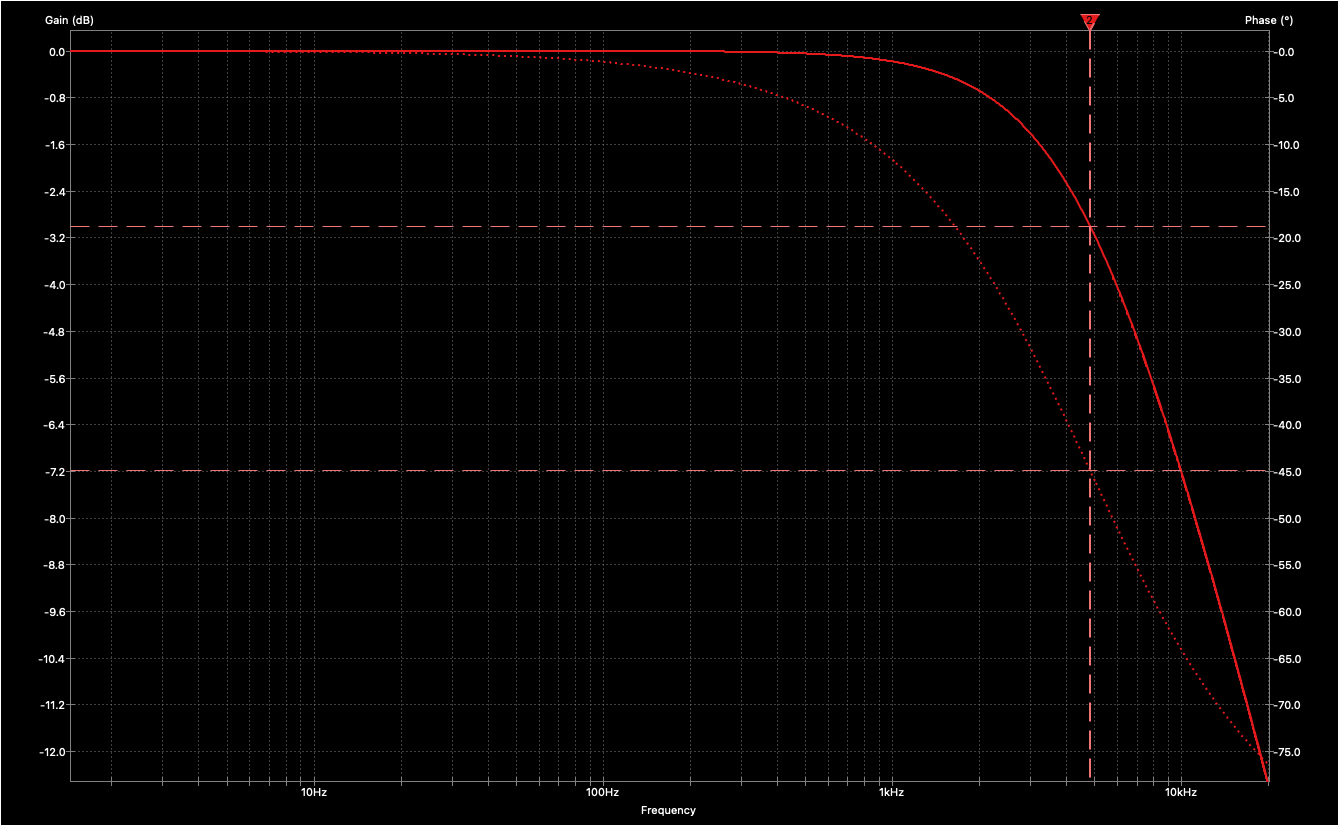
\includegraphics[width=1\textwidth]{Figures/Plots/Task3/3a-frekvens_plot.png}
    \figcaption{Frequency analysis of the circuit}
    \label{fig:Fplot3}
\end{figure}

Reading the plot at the point where the gain is at \(-3 \unit{dB}\), the resulting values for frequency and phase are found and listed in Table~\ref{tab:3a}.

% Table generated by Excel2LaTeX from sheet 'Part 3'
\begin{table}[htbp]
  \centering
  \tabcaption{Readings from plot}
    \begin{tabular}{|c|c|c|}
    \hline
    Frequency & Gain  & Phase \bigstrut\\
    \hline
    4,81kHz & -3dB  & -44,923° \bigstrut\\
    \hline
    \end{tabular}%
  \label{tab:3a}%
\end{table}%

\clearpage
\subsection{b}

\(F_{critical}\) is the point where the resistance is equal to the reactance, setting these equal each other, derives Equation~\ref{eq:f_C}. Using the known values of \(R\) and \(C\) the theoretical value was calculated and the simulated value was compared to it to find the deviation, listing the results in Table~\ref{tab:3b}.

\begin{equation*}
    X_C = \frac{1}{2 \pi f C}
\end{equation*}

\begin{equation*}
    R = X_C, \text{ at } f = F_{critical}
\end{equation*}

\begin{equation*}
    R = \frac{1}{2 \pi F_{critical} C}
\end{equation*}

\begin{equation}
    F_{critical} = \frac{1}{2 \pi R C}
    \label{eq:f_C}
\end{equation}

% Table generated by Excel2LaTeX from sheet 'Part 3'
\begin{table}[htbp]
  \centering
  \tabcaption{Calculated vs Simulated frequency}
    \begin{tabular}{|c|c|c|}
    \hline
    Calculated & Simulated & Deviation \bigstrut\\
    \hline
    4,82kHz & 4,81kHz & -0,27\% \bigstrut\\
    \hline
    \end{tabular}%
  \label{tab:3b}%
\end{table}%

\clearpage
\subsection{c}

Performing a transient analysis using the simulated \(F_{critical}\) value, the resulting plot is shown in Figure~\ref{fig:Tplot3c}.

\begin{figure}[h]
    \centering
    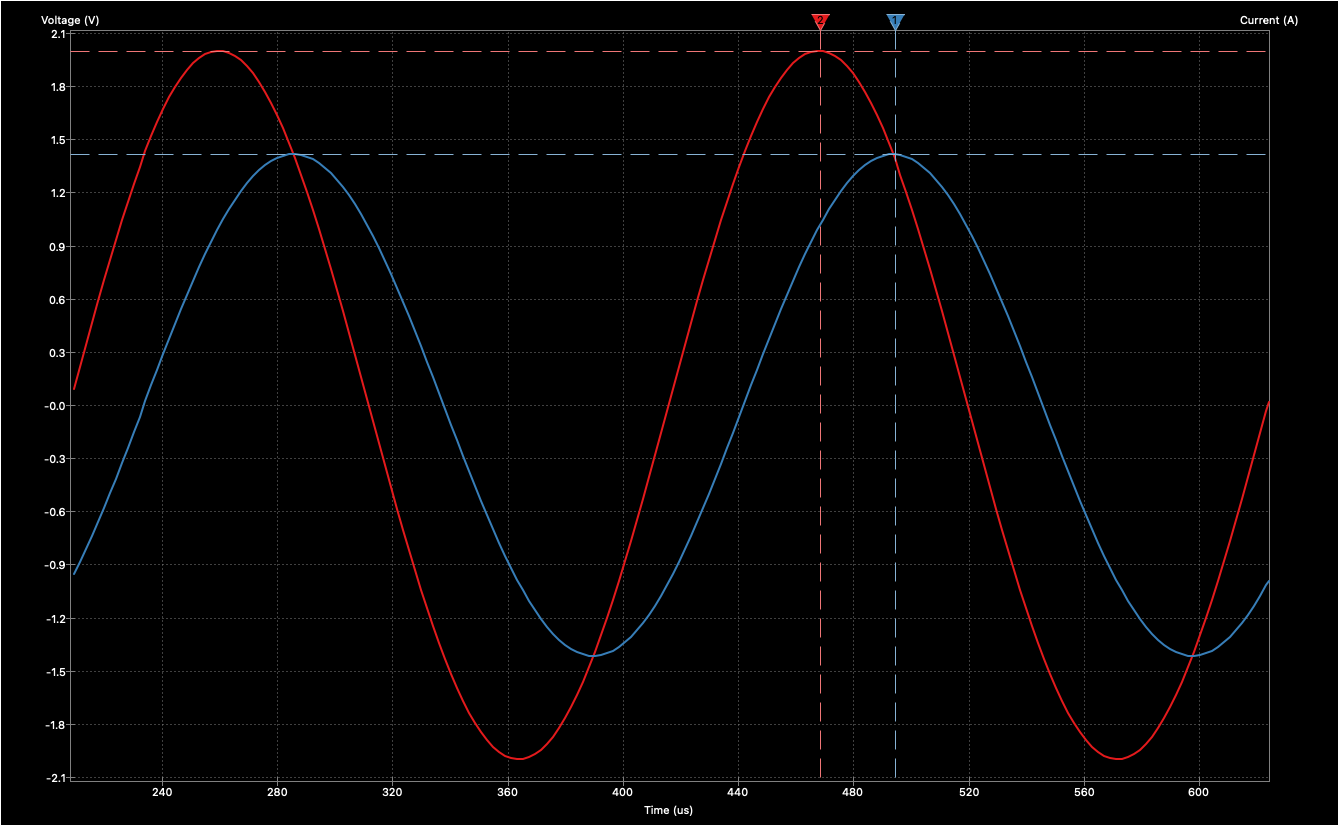
\includegraphics[width=1\textwidth]{Figures/Plots/Task3/3c-transient_plot.png}
    \figcaption{Transient analysis for 4,81kHz}
    \label{fig:Tplot3c}
\end{figure}

Reading the plot at the peak voltages, the resulting values and difference listed in Table~\ref{tab:3c}.

% Table generated by Excel2LaTeX from sheet 'Part 3'
\begin{table}[htbp]
  \centering
  \tabcaption{Simulated Voltages at 4,81kHz}
    \begin{tabular}{|c|c|c|}
    \hline
    \rowcolor[rgb]{ .753,  .902,  .961} Generator & \cellcolor[rgb]{ 1,  .592,  .584}Output & \cellcolor[rgb]{ 1,  1,  1}Difference \bigstrut\\
    \hline
    \rowcolor[rgb]{ .753,  .902,  .961} 2,00V & \cellcolor[rgb]{ 1,  .592,  .584}1,42V & \cellcolor[rgb]{ 1,  1,  1}583mV \bigstrut\\
    \hline
    \end{tabular}%
  \label{tab:3c}%
\end{table}%

\clearpage
\subsection{d}

Performing a transient analysis using a decade lower frequency than the simulated \(F_{critical}\) value, the resulting plot is shown in Figure~\ref{fig:Tplot3d}.

\begin{figure}[h]
    \centering
    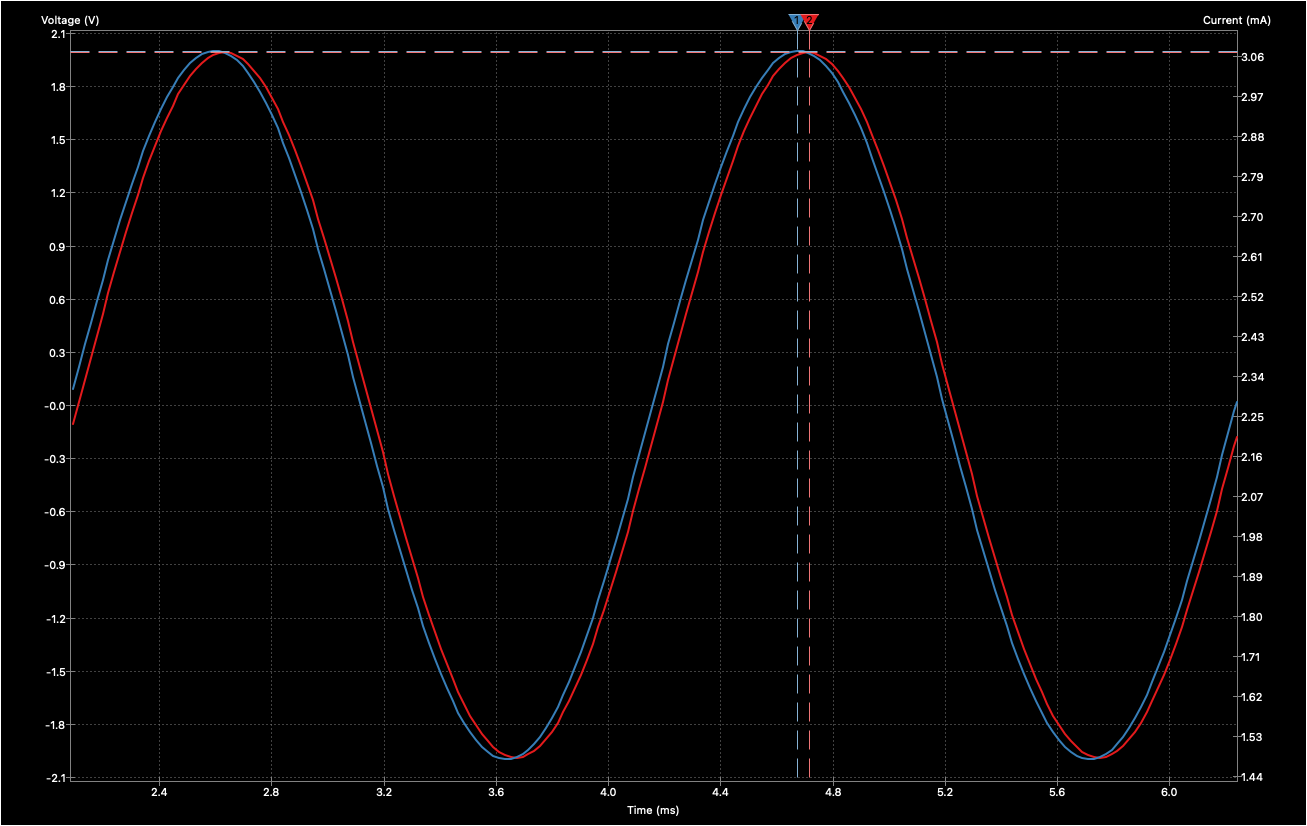
\includegraphics[width=1\textwidth]{Figures/Plots/Task3/3d-transient_plot.png}
    \figcaption{Transient analysis for 481Hz}
    \label{fig:Tplot3d}
\end{figure}

Reading the plot at the peak voltages, the resulting values and difference listed in Table~\ref{tab:3d}.

% Table generated by Excel2LaTeX from sheet 'Part 3'
\begin{table}[htbp]
  \centering
  \tabcaption{Simulated voltages at 481Hz}
    \begin{tabular}{|c|c|c|}
    \hline
    \rowcolor[rgb]{ .753,  .902,  .961} Generator & \cellcolor[rgb]{ 1,  .592,  .584}Output & \cellcolor[rgb]{ 1,  1,  1}Difference \bigstrut\\
    \hline
    \rowcolor[rgb]{ .753,  .902,  .961} 2,00V & \cellcolor[rgb]{ 1,  .592,  .584}1,99V & \cellcolor[rgb]{ 1,  1,  1}9,61mV \bigstrut\\
    \hline
    \end{tabular}%
  \label{tab:3d}%
\end{table}%

\clearpage
\subsection{e}

Performing a transient analysis using a decade higher frequency than the simulated \(F_{critical}\) value, the resulting plot is shown in Figure~\ref{fig:Tplot3e}.

\begin{figure}[h]
    \centering
    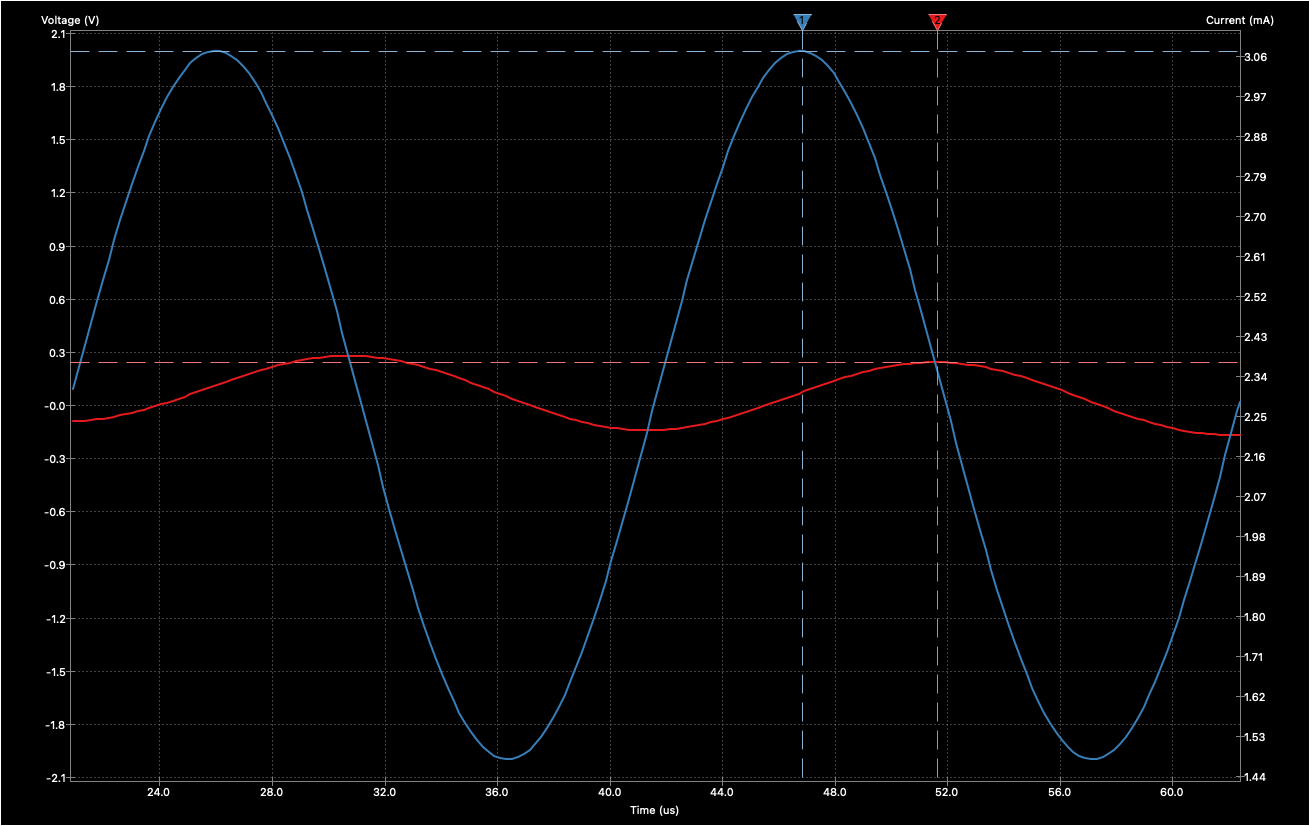
\includegraphics[width=1\textwidth]{Figures/Plots/Task3/3e-transient_plot.png}
    \figcaption{Transient analysis for 48,1kHz}
    \label{fig:Tplot3e}
\end{figure}

Reading the plot at the peak voltages, the resulting values and difference listed in Table~\ref{tab:3e}.

% Table generated by Excel2LaTeX from sheet 'Part 3'
\begin{table}[htbp]
  \centering
  \tabcaption{Simulated voltages at 48,1kHz}
    \begin{tabular}{|c|c|c|}
    \hline
    \rowcolor[rgb]{ .753,  .902,  .961} Generator & \cellcolor[rgb]{ 1,  .592,  .584}Output & \cellcolor[rgb]{ 1,  1,  1}Difference \bigstrut\\
    \hline
    \rowcolor[rgb]{ .753,  .902,  .961} 2,00V & \cellcolor[rgb]{ 1,  .592,  .584}241mV & \cellcolor[rgb]{ 1,  1,  1}1,76V \bigstrut\\
    \hline
    \end{tabular}%
  \label{tab:3e}%
\end{table}%

\subsection{f}
The values clearly show that the lower frequencies is almost not affected by the filer and the higher frequencies are drastically reduced, this means that this is a Low-pass filter.


%   ############################## Section ##############################
\section{Task 4}

In this task all simulations are done using the circuit in figure~\ref{fig:Circuit4}, the only thing changing is the frequency, based on the question.

\begin{figure}[h]
    \centering
    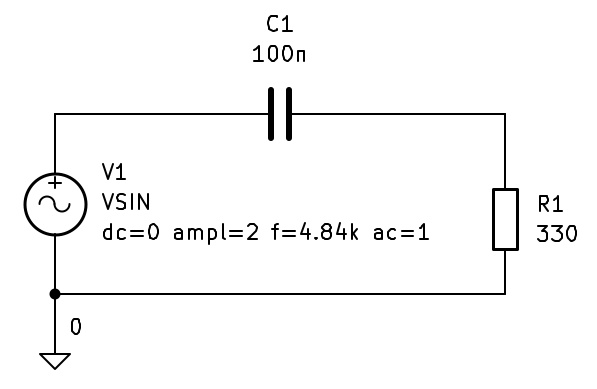
\includegraphics[width=0.8\textwidth]{Figures/Circuts/Task4.jpg}
    \figcaption{Circuit for Task 4}
    \label{fig:Circuit4}
\end{figure}

\clearpage
\subsection{a}

Doing a frequency analysis on the circuit gives the plot in Figure~\ref{fig:Fplot4}.

\begin{figure}[h]
    \centering
    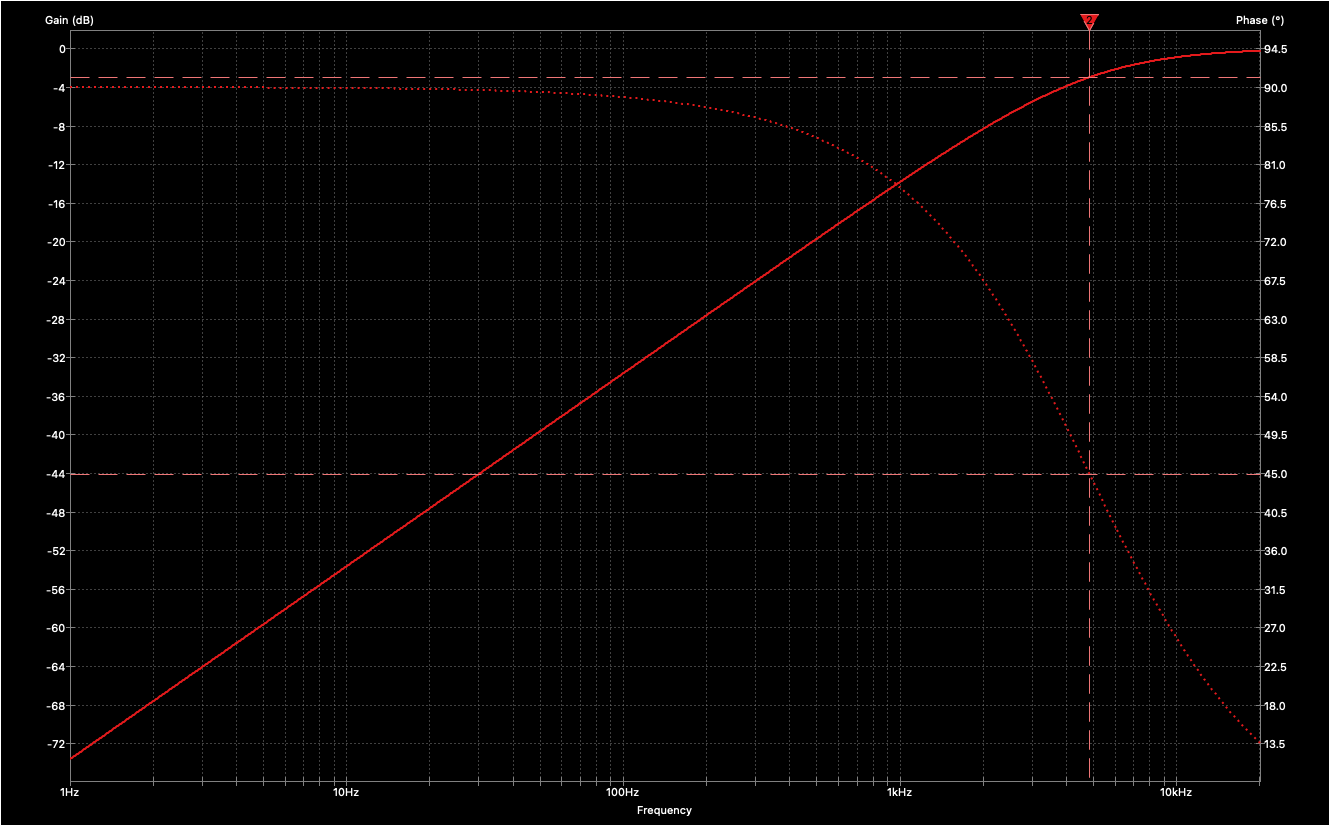
\includegraphics[width=1\textwidth]{Figures/Plots/Task4/4a-frekvens_plot.png}
    \figcaption{Frequency analysis of the circuit}
    \label{fig:Fplot4}
\end{figure}

Reading the plot at the point where the gain is at \(-3 \unit{dB}\), the resulting values for frequency and phase are found and listed in Table~\ref{tab:4a}.

% Table generated by Excel2LaTeX from sheet 'Part 4'
\begin{table}[htbp]
  \centering
  \tabcaption{Readings from plot}
    \begin{tabular}{|c|c|c|}
    \hline
    Frequency & Gain  & Phase \bigstrut\\
    \hline
    4,84kHz & -3dB  & 44,898° \bigstrut\\
    \hline
    \end{tabular}%
  \label{tab:4a}%
\end{table}%

\clearpage
\subsection{b}

Using the known values of \(R\) and \(C\) the theoretical value was calculated using Equation~\ref{eq:f_C}. Then the simulated value was compared to it to find the deviation, listing the results in Table~\ref{tab:4b}.

% Table generated by Excel2LaTeX from sheet 'Part 4'
\begin{table}[htbp]
  \centering
  \tabcaption{Calculated vs Simulated frequency}
    \begin{tabular}{|c|c|c|}
    \hline
    Calculated & Simulated & Deviation \bigstrut\\
    \hline
    4,82kHz & 4,84kHz & 0,36\% \bigstrut\\
    \hline
    \end{tabular}%
  \label{tab:4b}%
\end{table}%

\subsection{c}

Performing a transient analysis using the simulated \(F_{critical}\) value, the resulting plot is shown in Figure~\ref{fig:Tplot4c}.

\begin{figure}[h]
    \centering
    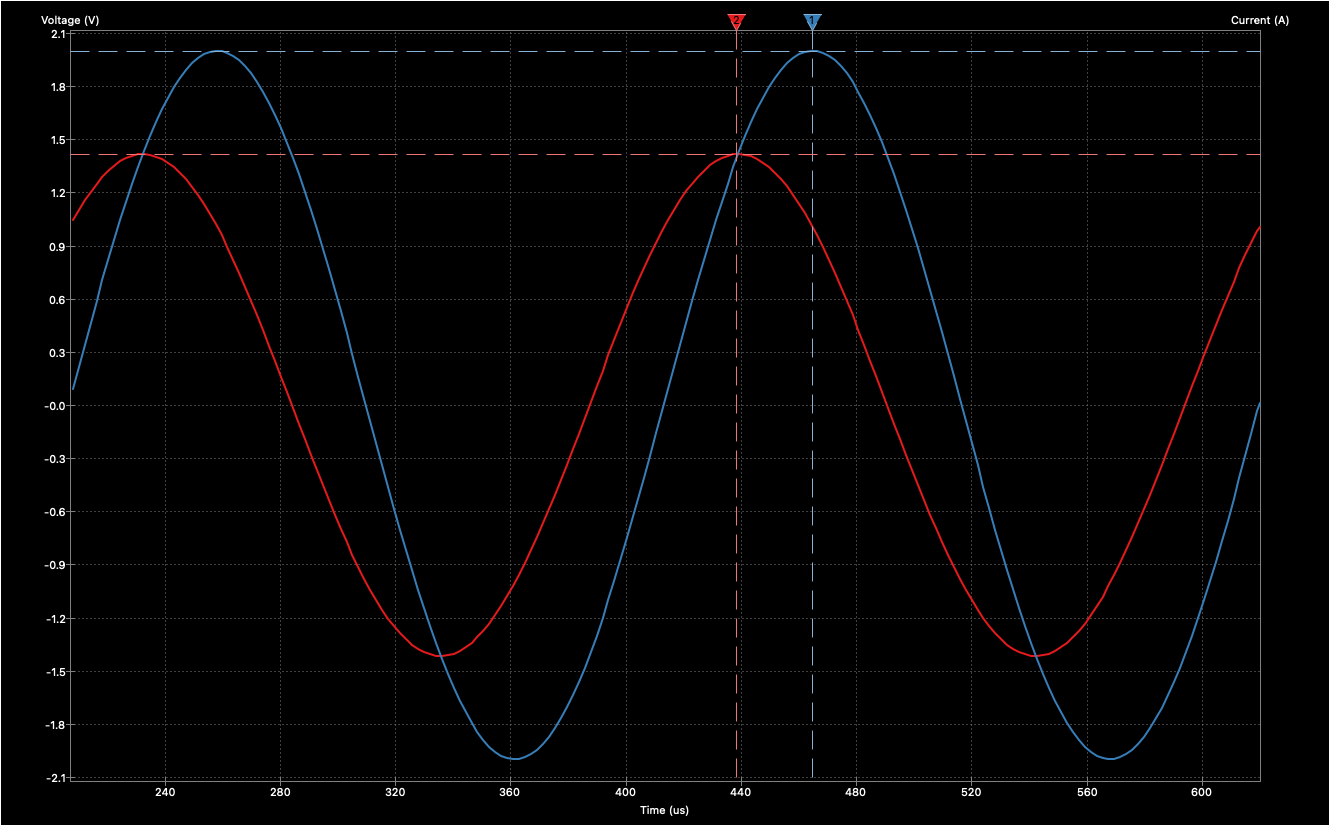
\includegraphics[width=1\textwidth]{Figures/Plots/Task4/4c-transient_plot.png}
    \figcaption{Transient analysis for 4,84kHz}
    \label{fig:Tplot4c}
\end{figure}

Reading the plot at the peak voltages, the resulting values and difference listed in Table~\ref{tab:4c}.

% Table generated by Excel2LaTeX from sheet 'Part 4'
\begin{table}[htbp]
  \centering
  \tabcaption{Simulated voltages at 4,84kHz}
    \begin{tabular}{|c|c|c|}
    \hline
    \rowcolor[rgb]{ .753,  .902,  .961} Generator & \cellcolor[rgb]{ 1,  .592,  .584}Output & \cellcolor[rgb]{ 1,  1,  1}Difference \bigstrut\\
    \hline
    \rowcolor[rgb]{ .753,  .902,  .961} 2,00V & \cellcolor[rgb]{ 1,  .592,  .584}1,42V & \cellcolor[rgb]{ 1,  1,  1}584mV \bigstrut\\
    \hline
    \end{tabular}%
  \label{tab:4c}%
\end{table}%

\clearpage
\subsection{d}

Performing a transient analysis using a decade lower frequency than the simulated \(F_{critical}\) value, the resulting plot is shown in Figure~\ref{fig:Tplot4d}.

\begin{figure}[h]
    \centering
    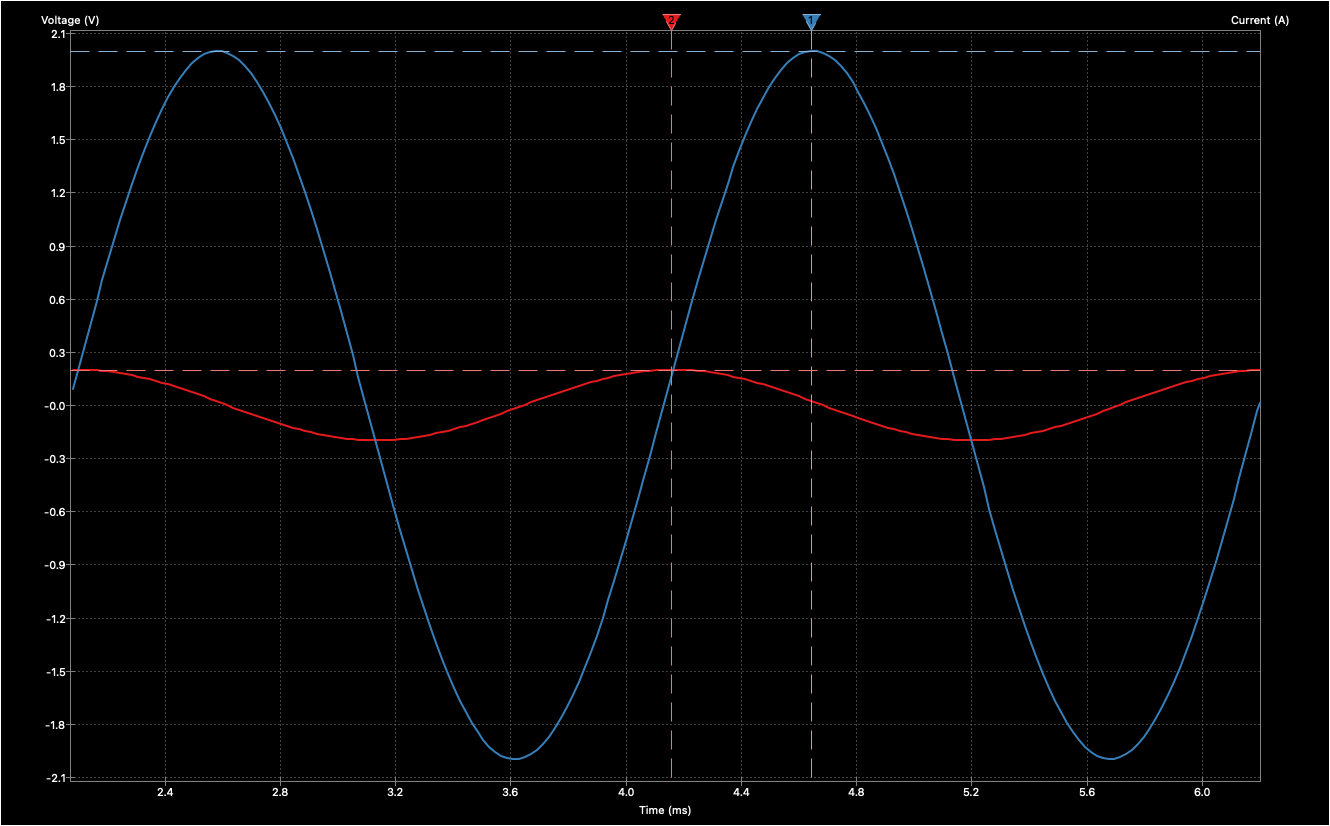
\includegraphics[width=1\textwidth]{Figures/Plots/Task4/4d-transient_plot.png}
    \figcaption{Transient analysis for 484Hz}
    \label{fig:Tplot4d}
\end{figure}

Reading the plot at the peak voltages, the resulting values and difference listed in Table~\ref{tab:4d}.

% Table generated by Excel2LaTeX from sheet 'Part 4'
\begin{table}[htbp]
  \centering
  \tabcaption{Simulated voltages at 484Hz}
    \begin{tabular}{|c|c|c|}
    \hline
    \rowcolor[rgb]{ .753,  .902,  .961} Generator & \cellcolor[rgb]{ 1,  .592,  .584}Output & \cellcolor[rgb]{ 1,  1,  1}Difference \bigstrut\\
    \hline
    \rowcolor[rgb]{ .753,  .902,  .961} 2,00V & \cellcolor[rgb]{ 1,  .592,  .584}200mV & \cellcolor[rgb]{ 1,  1,  1}1,8V \bigstrut\\
    \hline
    \end{tabular}%
  \label{tab:4d}%
\end{table}%

\clearpage
\subsection{e}

Performing a transient analysis using a decade higher frequency than the simulated \(F_{critical}\) value, the resulting plot is shown in Figure~\ref{fig:Tplot4e}.

\begin{figure}[h]
    \centering
    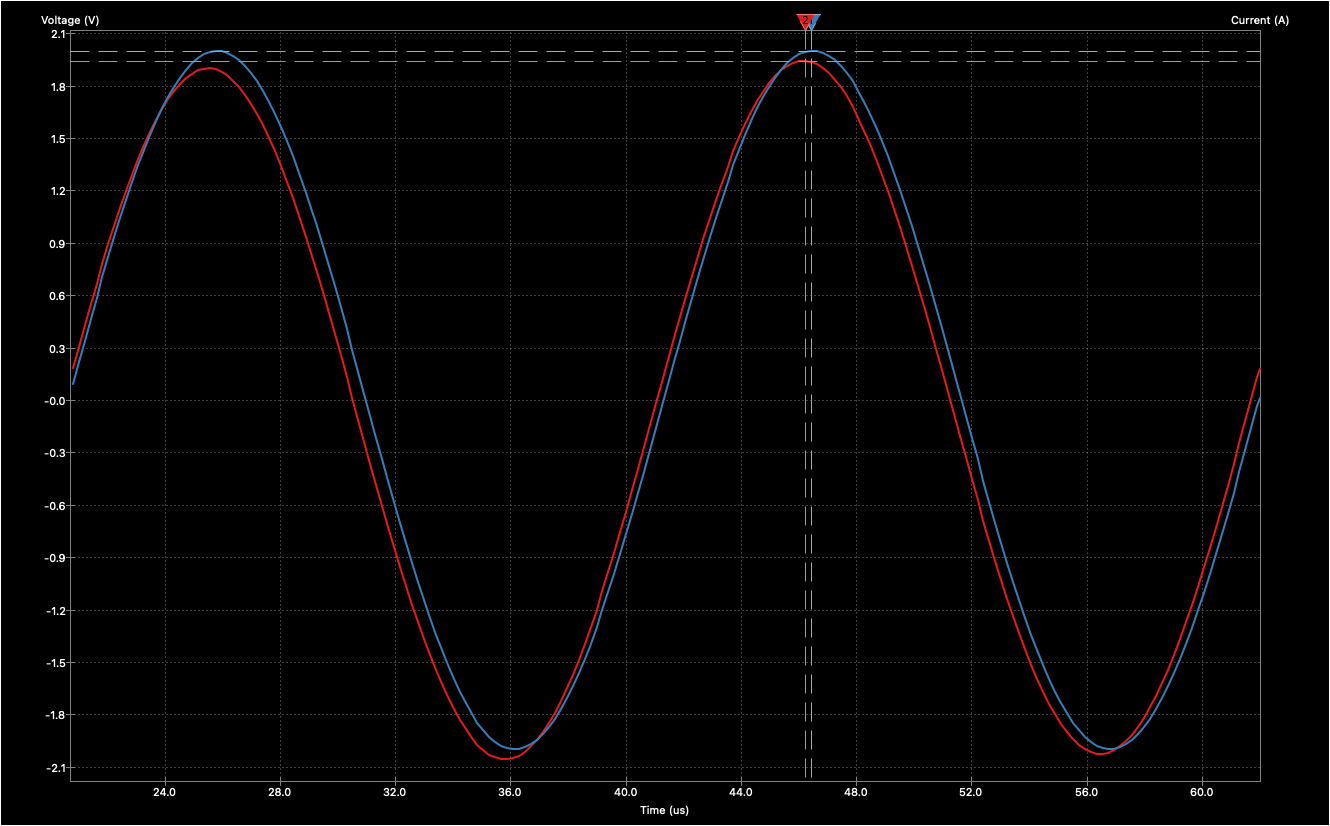
\includegraphics[width=1\textwidth]{Figures/Plots/Task4/4e-transient_plot.png}
    \figcaption{Transient analysis for 48,4kHz}
    \label{fig:Tplot4e}
\end{figure}

Reading the plot at the peak voltages, the resulting values and difference listed in Table~\ref{tab:4e}.

% Table generated by Excel2LaTeX from sheet 'Part 4'
\begin{table}[htbp]
  \centering
  \tabcaption{Simulated voltages at 48,4kHz}
    \begin{tabular}{|c|c|c|}
    \hline
    \rowcolor[rgb]{ .753,  .902,  .961} Generator & \cellcolor[rgb]{ 1,  .592,  .584}Output & \cellcolor[rgb]{ 1,  1,  1}Difference \bigstrut\\
    \hline
    \rowcolor[rgb]{ .753,  .902,  .961} 2,00V & \cellcolor[rgb]{ 1,  .592,  .584}1,94V & \cellcolor[rgb]{ 1,  1,  1}58,4mV \bigstrut\\
    \hline
    \end{tabular}%
  \label{tab:4e}%
\end{table}%

\subsection{f}

The values clearly show that the higher frequencies is almost not affected by the filer and the lower frequencies are drastically reduced, this means that this is a High-pass filter.


%   ############################## Section ##############################
\section{Task 5}

In this task all simulations are done using the circuit in figure~\ref{fig:Circuit5}, the only thing changing is the frequency, based on the question.

\begin{figure}[h]
    \centering
    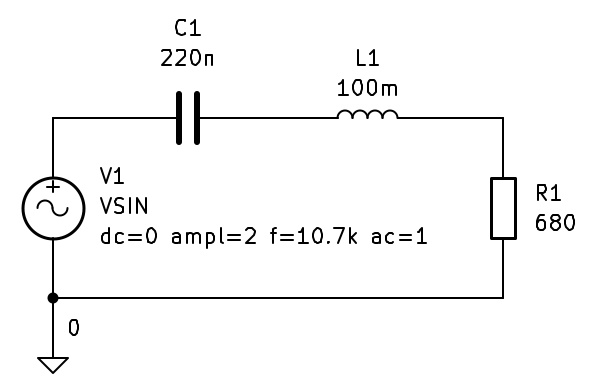
\includegraphics[width=0.8\textwidth]{Figures/Circuts/Task5.jpg}
    \figcaption{Circuit for Task 5}
    \label{fig:Circuit5}
\end{figure}

Note: This task was not supposed to be done as it was outside the scope of the Lab, therefore it  may be done incorrect. For one part, when there is both inductors and capacitors the formulas as used before do not apply. Instead of using the \(-3\unit{dB}\) point, the mid point was used as the "critical" frequency as by guidance from assistance this was the usual method of doing these types of tasks.

\clearpage
\subsection{a}

Doing a frequency analysis on the circuit gives the plot in Figure~\ref{fig:Fplot5}.

\begin{figure}[h]
    \centering
    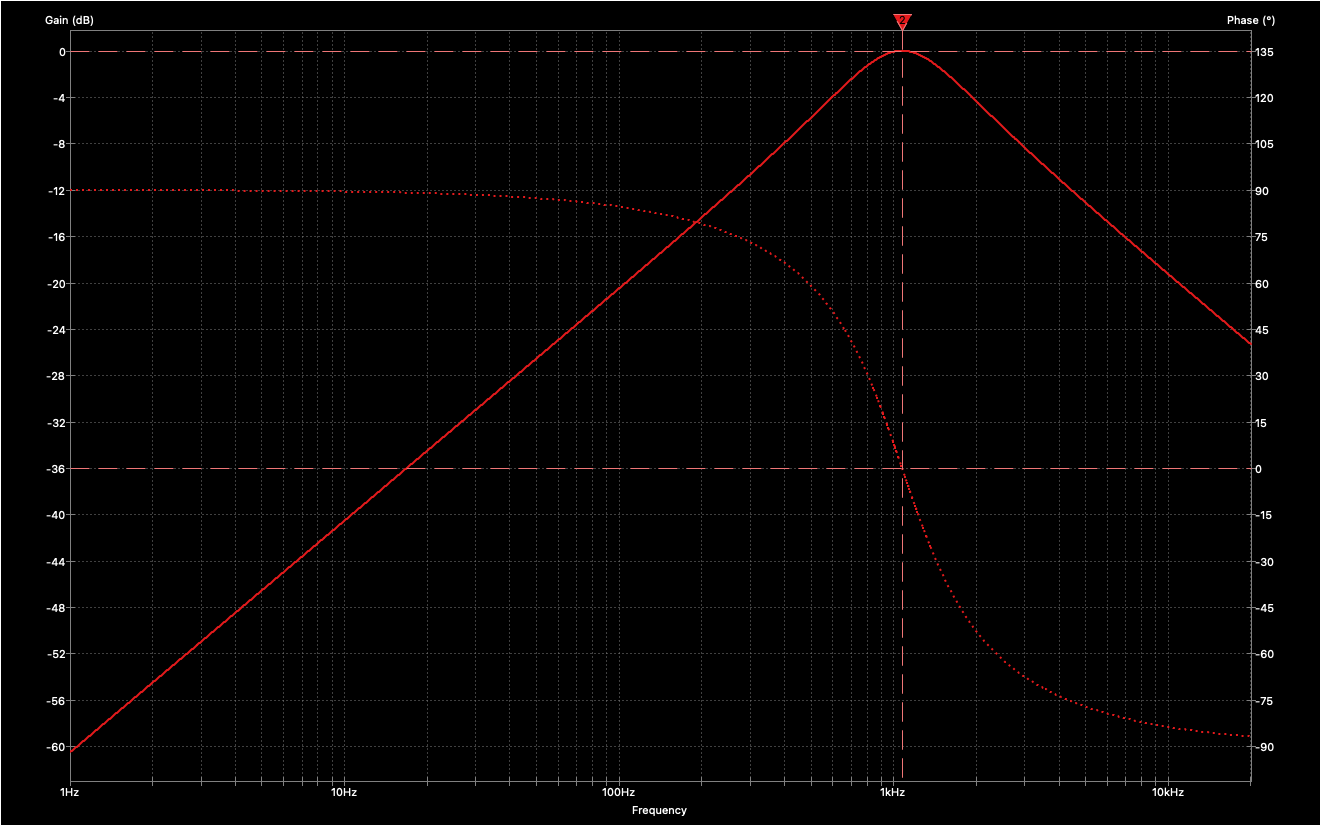
\includegraphics[width=1\textwidth]{Figures/Plots/Task5/5a-frekvens_plot_2center.png}
    \figcaption{Frequency analysis of the circuit}
    \label{fig:Fplot5}
\end{figure}

Reading the plot at the center point, the resulting values for frequency and phase are found and listed in Table~\ref{tab:5a}.

% Table generated by Excel2LaTeX from sheet 'Part 5'
\begin{table}[htbp]
  \centering
  \tabcaption{Readings from plot}
    \begin{tabular}{|c|c|c|}
    \hline
    Frequency & Gain  & Phase \bigstrut\\
    \hline
    1,07kHz & \approx 0 & \approx0° \bigstrut\\
    \hline
    \end{tabular}%
  \label{tab:5a}%
\end{table}%

\clearpage
\subsection{b}

\(F_{mid}\) is the point where the inductive reactance is equal to the capacitive reactance, setting these equal each other, derives Equation~\ref{eq:f_LC}. Using the known values of \(L\) and \(C\) the theoretical value was calculated and the simulated value was compared to it to find the deviation, listing the results in Table~\ref{tab:5b}.

\begin{equation*}
    X_L = 2 \pi f L
\end{equation*}

\begin{equation*}
    X_C = \frac{1}{2 \pi f C}
\end{equation*}

\begin{equation*}
    X_L = X_C, \text{ at } f = F_{mid}
\end{equation*}

\begin{equation*}
    2 \pi F_{mid} L = \frac{1}{2 \pi F_{mid} C}
\end{equation*}

\begin{equation*}
    F_{mid}^2 = \frac{1}{2^2 \pi^2 LC}
\end{equation*}

\begin{equation*}
    \sqrt{F_{mid}^2} = \sqrt{\frac{1}{2^2 \pi^2 LC}}
\end{equation*}

\begin{equation}
    F_{mid} = \frac{1}{2 \pi \sqrt{R C}}
    \label{eq:f_LC}
\end{equation}

% Table generated by Excel2LaTeX from sheet 'Part 5'
\begin{table}[htbp]
  \centering
  \tabcaption{Calculated vs Simulated frequency}
    \begin{tabular}{|c|c|c|}
    \hline
    Calculated & Simulated & Deviation \bigstrut\\
    \hline
    1,073kHz & 1,07kHz & -0,28\% \bigstrut\\
    \hline
    \end{tabular}%
  \label{tab:5b}%
\end{table}%

\clearpage
\subsection{c}

Performing a transient analysis using the simulated \(F_{mid}\) value, the resulting plot is shown in Figure~\ref{fig:Tplot5c}.

\begin{figure}[h]
    \centering
    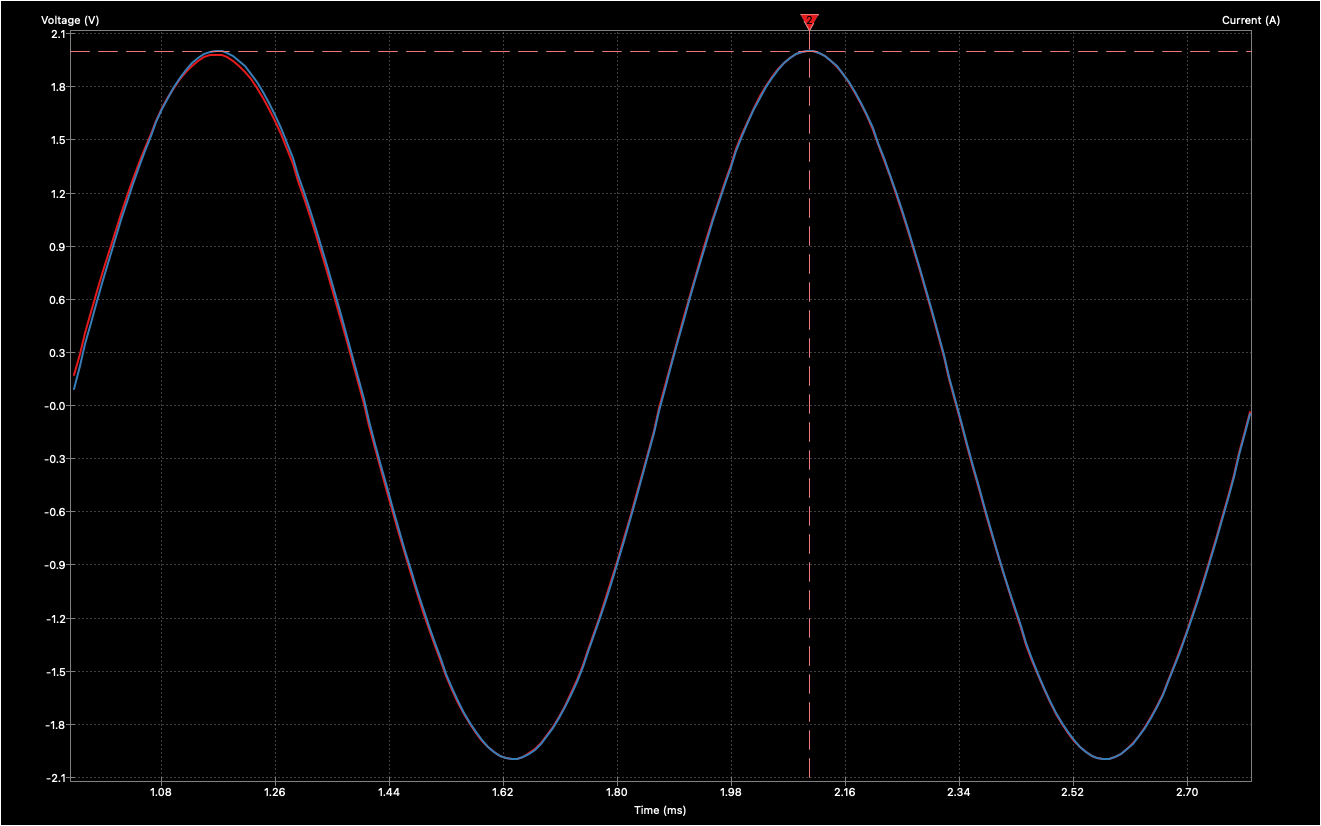
\includegraphics[width=1\textwidth]{Figures/Plots/Task5/5c-transient_plot.png}
    \figcaption{Transient analysis for 1,07kHz}
    \label{fig:Tplot5c}
\end{figure}

Reading the plot at the peak voltages, the resulting values and difference listed in Table~\ref{tab:5c}.

% Table generated by Excel2LaTeX from sheet 'Part 5'
\begin{table}[htbp]
  \centering
  \tabcaption{Simulated voltages at 1,07kHz}
    \begin{tabular}{|c|c|c|}
    \hline
    \rowcolor[rgb]{ .753,  .902,  .961} Generator & \cellcolor[rgb]{ 1,  .592,  .584}Output & \cellcolor[rgb]{ 1,  1,  1}Difference \bigstrut\\
    \hline
    \rowcolor[rgb]{ .753,  .902,  .961} 2,00V & \cellcolor[rgb]{ 1,  .592,  .584}2,00V & \cellcolor[rgb]{ 1,  1,  1}148µV \bigstrut\\
    \hline
    \end{tabular}%
  \label{tab:5c}%
\end{table}%

\clearpage
\subsection{d}

Performing a transient analysis using a decade lower frequency than the simulated \(F_{mid}\) value, the resulting plot is shown in Figure~\ref{fig:Tplot5d}.

\begin{figure}[h]
    \centering
    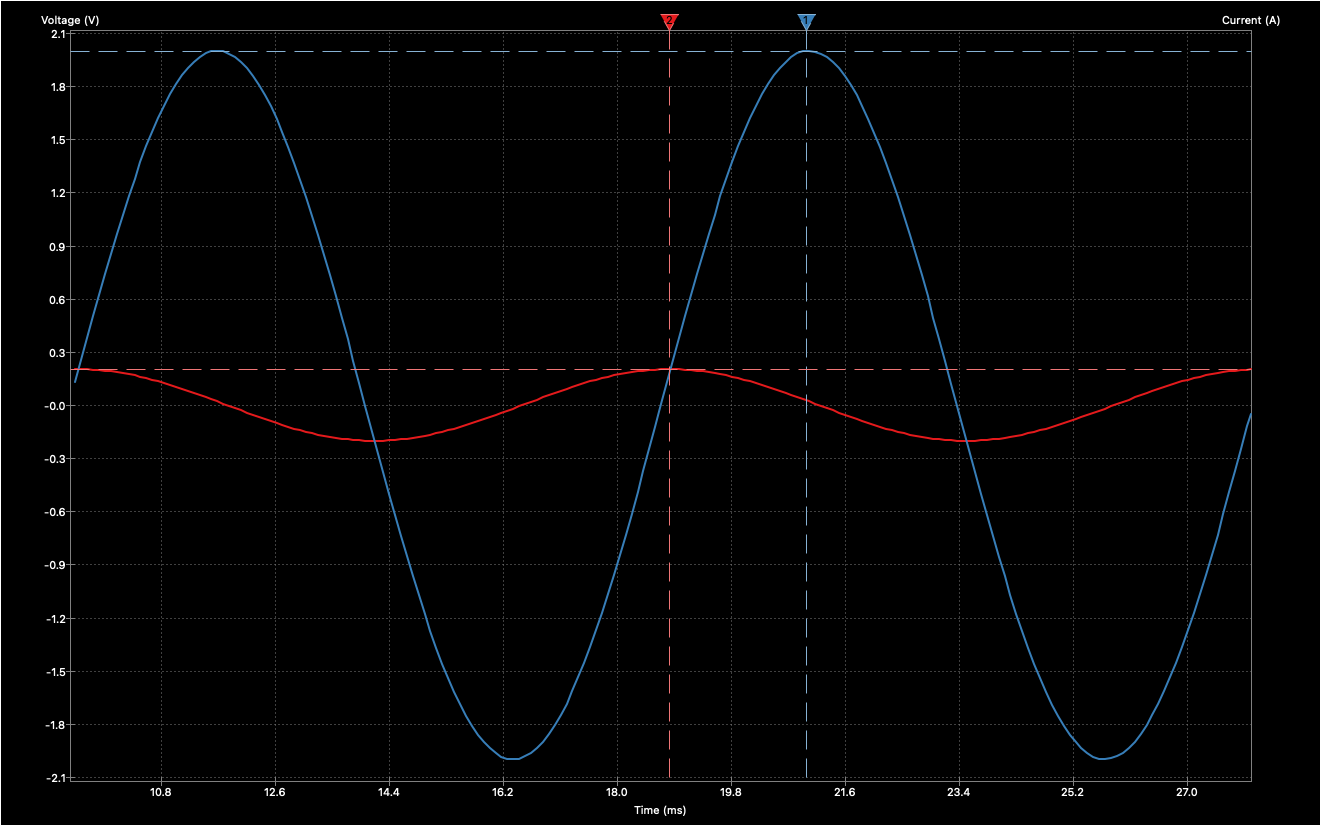
\includegraphics[width=1\textwidth]{Figures/Plots/Task5/5d-transient_plot.png}
    \figcaption{Transient analysis for 107Hz}
    \label{fig:Tplot5d}
\end{figure}

Reading the plot at the peak voltages, the resulting values and difference listed in Table~\ref{tab:5d}.

% Table generated by Excel2LaTeX from sheet 'Part 5'
\begin{table}[htbp]
  \centering
  \tabcaption{Simulated voltages at 107Hz}
    \begin{tabular}{|c|c|c|}
    \hline
    \rowcolor[rgb]{ .753,  .902,  .961} Generator & \cellcolor[rgb]{ 1,  .592,  .584}Output & \cellcolor[rgb]{ 1,  1,  1}Difference \bigstrut\\
    \hline
    \rowcolor[rgb]{ .753,  .902,  .961} 2,00V & \cellcolor[rgb]{ 1,  .592,  .584}202mV & \cellcolor[rgb]{ 1,  1,  1}1,8V \bigstrut\\
    \hline
    \end{tabular}%
  \label{tab:5d}%
\end{table}%

\clearpage
\subsection{e}

Performing a transient analysis using a decade higher frequency than the simulated \(F_{mid}\) value, the resulting plot is shown in Figure~\ref{fig:Tplot5e}.

\begin{figure}[h]
    \centering
    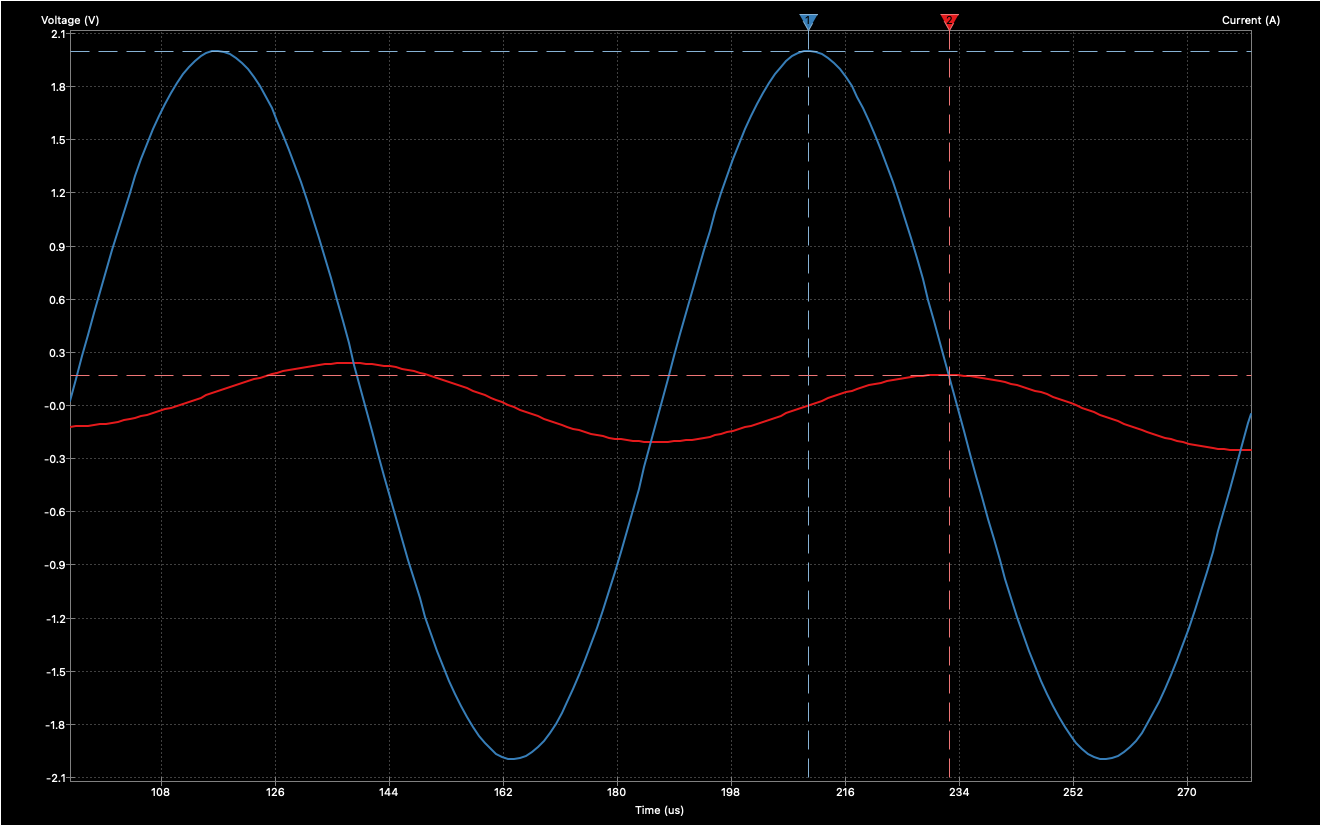
\includegraphics[width=1\textwidth]{Figures/Plots/Task5/5e-transient_plot.png}
    \figcaption{Transient analysis for 10,7kHz}
    \label{fig:Tplot5e}
\end{figure}

Reading the plot at the peak voltages, the resulting values and difference listed in Table~\ref{tab:5e}.

% Table generated by Excel2LaTeX from sheet 'Part 5'
\begin{table}[htbp]
  \centering
  \tabcaption{Simulated voltages at 10,7kHz}
    \begin{tabular}{|c|c|c|}
    \hline
    \rowcolor[rgb]{ .753,  .902,  .961} Generator & \cellcolor[rgb]{ 1,  .592,  .584}Output & \cellcolor[rgb]{ 1,  1,  1}Difference \bigstrut\\
    \hline
    \rowcolor[rgb]{ .753,  .902,  .961} 2,00V & \cellcolor[rgb]{ 1,  .592,  .584}170mV & \cellcolor[rgb]{ 1,  1,  1}1,83V \bigstrut\\
    \hline
    \end{tabular}%
  \label{tab:5e}%
\end{table}%

\subsection{f}

The values clearly show that the middle frequencies is almost not affected by the filer and the lower and higher frequencies are drastically reduced, this means that this is a Band-pass filter.


\end{document}